\documentclass[twoside,a4paper,12pt]{report}

\usepackage{a4wide}
\usepackage{epsfig}
\usepackage{amsmath}
\usepackage{amssymb}
%\usepackage{mathptmx}
\usepackage{latexsym}
\usepackage{epic}
\usepackage{eepic}
%\usepackage{axodraw}
\usepackage[small,it]{caption}
%\usepackage[flushmargin]{footmisc}
%\usepackage[marginal,symbol,perpage]{footmisc}
\usepackage[marginal]{footmisc}
\usepackage{pifont}

\setlength{\parskip}{12pt}  % 12 pt = space between paragraphs
\setlength{\parindent}{0pt} % 0 pt  = indentation
\setlength{\captionmargin}{1.5cm}
%\abovecaptionskip
%\belowcaptionskip

\begin{document}

\begin{titlepage}
\begin{center}
  \phantom{A}
  \vspace{0.2cm}
  {\bf \Huge Monte-Carlo Simulations \\[1mm]
  of\\[5mm] Atoms} \\
  \vspace{1.5cm}
  {\bf \large Cand.\ Scient.\ Thesis in Theoretical Many-Body Physics} \\
  \vspace{0.5cm}
  {\bf \large by \\[5mm] Simen S. Reine} \\
  \vspace{2cm}
%  \includegraphics[width=5cm]{figs/ugle.eps} \\
  \vspace{2cm}
  {\bf Department of Physics \\ University of Oslo \\ Norway}\\
  \vspace{1.5cm}
  {\bf December 2003} \\
\end{center}
\end{titlepage}

\clearpage
\thispagestyle{empty}
\cleardoublepage
\pagestyle{headings}
\pagenumbering{roman}      % i,ii,iii,iv...


\documentclass[../main.tex]{subfiles}
 
\begin{document}
%\thispagestyle{empty}
I first discovered physics during high school, thanks to my brother Alexander Fleischer. He knew how much I liked mathematics, so he recommended a course in physics to me. I ended up liking it even more than mathematics, and as a result, after high school I applied to the physics, meteorology and astronomy Bachelor program at the University of Oslo.

The very first semester I was introduced to a field I liked just as much as physics, namely programming. Unfortunately, my Bachelor did not involve much programming after the first year. During the third year I had the option of taking an introductory course in computational physics, but I had several other physics courses I wanted to take, and I prioritized these over computational physics.

When it was time to apply for a Masters program, I was unsure of what to pick. I then remembered how fun all the programming had been during the first year, and decided to give the combination of physics and programming a try, so I applied to the computational physics Masters program. The first semester I took the introductory computational physics course, and knew immediately that I had picked the right Masters program for me.

I would like to thank my supervisor Morten Hjorth-Jensen for all the help and motivation he gave me during the past two years. I would also like to thank my brother Alexander for introducing me to physics in the first place, and for the helpful discussions we had about this thesis. 

Additionally, I would like to thank Håkon V. Treider for the fun times we have had sharing an office for the better part of two years, and for the help he has given me with general programming related issues. Finally, I would like to thank the various other people I shared an office with over the past two years, and the rest of the people at the computational physics research group, for making it a great place to be.

{\raggedleft\vfill\itshape\Longstack[l]{%
  Christian Fleischer\\
  Oslo, May 2017
}\par
}

\end{document}


\clearpage
\setlength{\parskip}{0pt}  % 0 pt = space between paragraphs
\tableofcontents
\thispagestyle{plain}

\clearpage


\pagenumbering{arabic}     % 1,2,3,4,...
\chapter{Introduction}
\label{introduction}

\section{Historical Background}

About 2400 years ago, the Greek philosopher Anaxagoras invented the
idea that matter could be devided into infinitly small parts;
\emph{spermata}. 
This concept was expanded a few years later by
Democritus, who believed matter was composed of tiny particles of
finite size or mass. He called the invisible particles of matter
\emph{atoms}; which in greek means 'undevidable'. 
No experimental techniques needed to test the atomic
hypotheses existed at the time, and there was no advance in the
understanding of atoms for more than 2000 years! 

\subsection*{Discovery of the Atom}

In 1807, John Dalton postulated that atoms of each element had a
unique mass. Dalton's atomic theory contained a simple prediction for
the case where two elements combine to form two different compounds;
\emph{The Law of Multiple Proportions}. (For example, 16 g of oxygen, O,
combines with 12 g of carbon, C, to form carbonmonoxide, CO, and
32 g of O combines with 12 g of C to form carbondioxide, CO$_2$).
%
\newline
%
A great leap in the understanding of the structure of matter was made
in 1811 by Amedeo Avogadro. Avogadro correctly hypothesized that the
particles of a gas were small compared to the distance between the
particles. He determined that these particles were often made up of
more than one atom; \emph{molecules}. This important result is the
basis for the \emph{Ideal Gas Law}, and the discovery provided a
systematic method for measurement of the atomic mass numbers.

\subsection*{The Periodic Table}

In 1869, Dmitri Mendeleev made the first classification of the
elements. The elements were ordered with increasing atomic mass
number, and placed in several columns according to their chemical
properties. Mendeleev discovered some gaps, that made him to correctly
predict the existance of undiscovered elements!

\subsection*{Discovery of the Electron}

A type of radiation, called \emph{cathode rays}, was observed to be
emitted from metallic surfaces when voltage was applied. At the end of
the 19$^{th}$ century there was much speculation about the fundamental
properties of the cathode rays. One school of thought held the belief
that cathode rays were particles, while the other school believed it
was a wave-phenomenon. In 1897, Joseph John Thomson preformed a
definitive set of experiments that proved that cathode rays had
a particle behavior. Thomson developed the necessary technique to
observe the deflection of chatode rays in an electric field. This led
to the interpretation of chatode rays as charged particles;
\emph{electrons}.

\subsection*{Measurement of the Electric Charge}

In 1909, Robert Millikan made the first accurate measurement of the
electron charge. \emph{The Millikan Oil-Droplet Experiment} was
performed by spraying tiny droplets of oil between two conducting
plates. By switching the electric field between the two plates on and
off, Millikan was able to accuratly estimate the electron charge. The
result of numerous measurements by Millikan, was that the charge was
allways an integer multiple of $1.6 \cdot 10^{-19}C$.
Figure \ref{oil_droplet} illustrates the forces acting on the
oil-droplet.

\begin{figure}[hbtp]
\begin{center}
  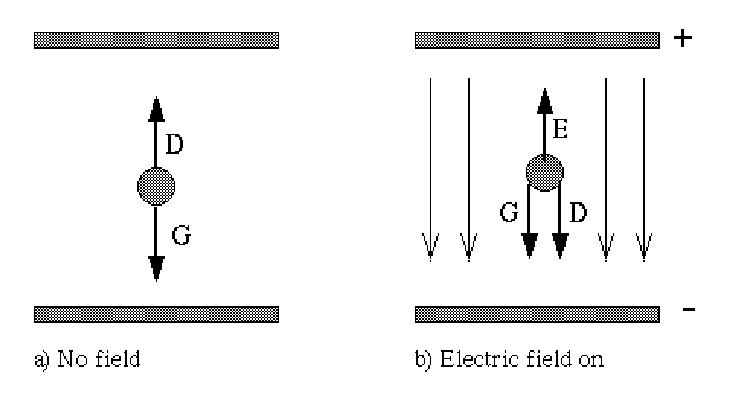
\epsfig{file=Introduction/oil_droplet.eps, height=5cm}
  \caption{
    Forces on an oil-droplet in: \newline
    \hspace*{1.5cm}
           a) Free fall          \newline
    \hspace*{1.5cm}
	   b) Electric field     \newline
    (G=Gravitation, D=Drag, E=Electric force)
  }
  \label{oil_droplet}
\end{center}
\end{figure}

His results were systematically low by about 4\% due to inaccurate
knowledge of the coefficient of viscosity. \newline
The electron charge is -e,
where $e = 1.602 \cdot 10^{-19}C$. All free particles are observed to
have values of electric charge equal to an integer times the
fundamental charge e:

\begin{equation*}
  q=n e
\end{equation*}

where the integer $n=\dots,-1,0,1,\dots$ is the electric charge
\emph{quantum number}.

\subsection*{The Nucleus}

In 1912, Ernest Rutherford and his associates discovered that the
positive charge of the atom is concentrated in a \emph{nucleus}. The
charge of the $\alpha$ particle, discovered by Becquerel, was
determined to be $2e$, and the mass of the $\alpha$ particle was
determined to be about four times the mass of the hydrogen
atom. \newline
A new particle with zero electric charge was discovered by bombarding
beryllium atoms with $\alpha$ particles. James Chadwick showed that
the new particle, the \emph{neutron}, had mass nearly equal to that of
the \emph{proton}.

\subsection*{The Bohr Model of the Atom}

In 1913, Niels Bohr made the first qunatitatively successful model of
the atom. Inspired by the work of Rutherford, Bohr made a planetary
model of the atom; with electrons moving in circular orbits about the
nucleus. This model may seem quite simple in retrospect, but for the
time it was a great advancement of science. In addition to the
classical circular orbits, the second part of Bohr's atomic model
contains a bold hypothesis of new physics. The new physics recognizes
that \emph{angular momentum} is \emph{quantized}; it can take only
certain values:

\begin{equation*}
  L = mvr = n \hbar
\end{equation*}

where $n$ is a positive integer. Solving the energy equations result
in orbits of radius:

\begin{equation*}
  r_n = \frac{n^2\hbar^2}{mke^2}
\end{equation*}

where the \emph{Bohr radius}

\begin{equation*}
  a_0 \equiv r_1 = \frac{\hbar^2}{mke^2} \approx 0.053 nm
\end{equation*}

is in the correct order of magnitude for the size of the atom!

{\bf Planc }


\clearpage

\chapter{The Basis of Quantum Mechanics}

%**************** From Classical of Quantum Mechanics *************
%
\section{Introduction to Quantum Mechanics}

In this section we will give a brief introduction to some of the basic
properties of quantum mechanics. For a more thourough introduction to
quantum mechanics there are several references, among other
\cite{rohlf1994}, \cite{shankar1994} and \cite{hemmer1980}.

%*                    Wave-Particle Duality                    *
\subsection{Wave-Particle Duality}

Let us start out with a simple experiment. We send light through a
tiny\footnote{With 'tiny' we mean the approximate size of
the light's wave-length.} slit, and observe the
intensity-pattern on a screen behind the slit. The pattern is
illustrated in figure \ref{singleSlit}.

\begin{figure}[hbtp]
\begin{center}
  \epsfig{file=Basic_QM/singleSlit.eps, height=6cm}
  \caption{
    Single-slit diffraction
  }
  \label{singleSlit}
\end{center}
\end{figure}

We now expand the above experiment to include two slits, and get an
interference pattern as that given by figure \ref{doubleSlit}. 

\begin{figure}[hbtp]
\begin{center}
  \epsfig{file=Basic_QM/doubleSlit.eps, height=9cm}
  \caption{
    Double-slit diffraction
  }
  \label{doubleSlit}
\end{center}
\end{figure}

If we sent classical particles through a double slit we would expect a
superposition of two single-slit intensity patterns. But this is not
what we actually observe for light.

In addition to the observed diffraction of light,
light may also be reflected and refracted. The reflection of light creates
the mirror image of a mountain on a still lake, and the light of
the sun refracted by a prism creates the rainbow hues. All the above
indicates that light has a wave-behavior. 
\newline
%
\newline

Lets us continue with yet another experiment. We direct light at a
conductive surface as illustrated in figure
\ref{photoElectricEffect}. 

\begin{figure}[hbtp]
\begin{center}
  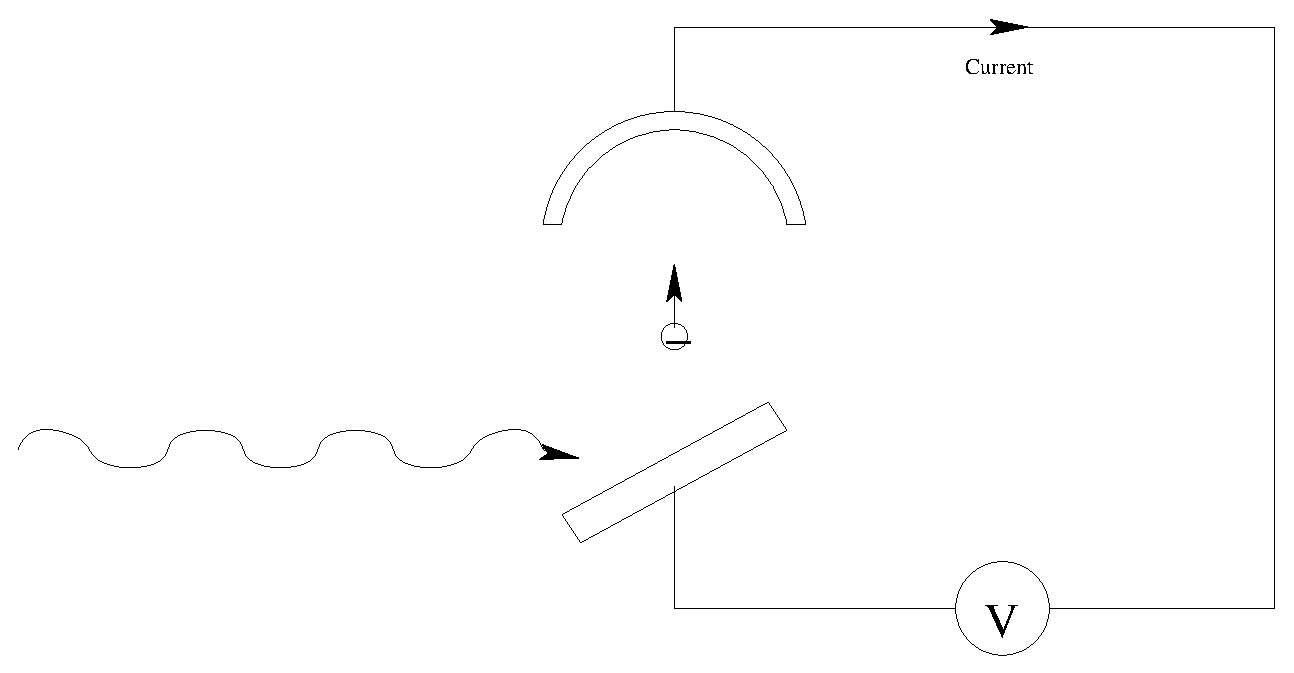
\epsfig{file=Basic_QM/photoElectricEffect.eps, height=6cm}
  \caption{
    Photo-electric effect
  }
  \label{photoElectricEffect}
\end{center}
\end{figure}


The light induces both a voltage and a current in the electric
circuit. What now if we increase the intensity of light? If light
were waves we would expect the voltage to increase, but only the
current is increased. This would indicate that light transfers only a
limited (even quantized!) amount of kinetic energy to the
electrons. But how can this be if light are waves? Who knows, but it's
in the nature of light. Furthermore, there is a lower limit of the
frequency needed to induce the photo-electric effect, dependent on the
photo-cathodic surface the light is directed at. Finally, if light
were waves, we would expect some time delay between when the light
source is turned on and the photo-electric effect is induced, but no
such delay is observed.

We have shown that light has both wave and particle
behavior, and this \emph{wave-particle duality} has no explanation in
classical physics. This duality is present in all objects, but is
measurable only for (sufficiently) small 'particles'.
\newline
%
\newline
%*                          DeBroglie Waves                       *
%\subsection{DeBroglie Waves}

In 1905 Einstein proposed that light has particle properties, 
and that each \emph{quanta} of light ({\bf photon}) has energy
  proportional to its frequency, $\nu$, 

\begin{equation*}
  E = h \nu
\end{equation*}

Here Planck's constant $h=6.626 \cdot 10^{-34} J \cdot s$, is a
fundamental constant of nature. Also in 1905, Einstein demonstrated, in
his special theory of relativity, that the photon has momentum like a
particle  

\begin{equation*}
  p = \frac{h} {\lambda}
\end{equation*}

This idea was generalized by Louis De Broglie, when he in 1924 proposed
that all matter have wave-like properties, and that they thus have a
wavelength ({\bf De Broglie wavelength}), 

\begin{equation*}
  \lambda = \frac{h} {p}
\end{equation*}



%*             Heisenberg's Uncertainty Principle             *
\subsection{Heisenberg's Uncertainty Principle}

In 1925 Heisenberg formulated his {\bf Uncertainty
  Principle}. Heisenberg's uncertainty principle states that one cannot
  measure a particle's position and momentum simultaneously with
  infinite precision.

\begin{equation*}
  \Delta x \Delta p \ge \frac{\hbar}{2}
\end{equation*}

Here $\Delta x$ and $\Delta p$ are the uncertainties in the position
and the momentum, respectively, and the \emph{reduced Plank's constant}
$\hbar = h/2\pi$. Also,

\begin{equation*}
  \Delta E \Delta t \ge \frac{\hbar}{2}
\end{equation*}

where $\Delta E$ and $\Delta t$ are the uncertainties energy and time,
respectively.

A consequence of the uncertainty principle is that
measuring the state of a microscopic system changes the system. 
\newline
%
\newline

Consider the double-slit experiment, depicted in figure
\ref{doubleSlit}, and reduce the intensity to allow only one
particle's to pass the slit at a time. What now? The interference
pattern in the figure now represents the particle's probability
distribution function. But how is this possible? In the classical way
of thinking the particle either passes the upper or the lower
slit. Following this line of thinking would lead to the superposition
of two single-slit experiments. This is not the case! So what then is
the solution? Either the photon is emitted from it's source at one
time, and then moves through both slits at the same time before
hitting the screen, or one simply cannot talk about a path at all.
Who knows?

So what then is the physicists approach?



%*                           The Quantum State                          *
\subsection{The Quantum State}

A proper description of a state allows all the known properties of
a system to be found. For a macroscopic system, the state of a
particle at a given time can be specified by a point in 
{\bf phase space}, i.e. the space spanned by the spatial coordinates
and the momentum coordinates. The energy, spin etc. of a particle, may 
all be found from the state of the particle.

In 1926 Erwin Schr\"odinger developed the idea of the \emph{complex}
{\bf wave function}, $\Psi = \Psi (\mathbf{x},t)$,
which is the state of microscopic systems. Unlike a trajectory the
wave-function has no independent reality. It only bears meaning in
conjunction with its complex conjugate $\Psi^*$ and an {\bf
  operator}. For example $\Psi^* \Psi = |\Psi|^2$ 
may be interpreted as a {\bf probability density} (here the operator
is the identity). For a given time
$t$ this has physical meaning when associated with a region in
space. Furthermore, this interpretation implies that the norm

\begin{equation*}
  \int\limits_{\Omega} |\Psi|^2 d\Omega = 1
\end{equation*}

where $\Omega$ is space. Thus, the wave-function must be
normalizable. 



%*                  Operators and Observables                          *
\subsection{Operators and Observables}

Every {\bf observable} (or measurable quantity) has an operator. The
information available in a wave-function is extracted by using the
operator to calculate an {\bf expectation value}. The expectation
value of an operator, $\left< \hat{{\cal O}} \right>$, is defined as

\begin{equation*}
  \left< \hat{{\cal O}} \right> 
  = \frac {\int \Psi^* \hat{{\cal O}} \Psi}  {\Psi^* \Psi}
\end{equation*}

For each classical variable
$\omega(\mathbf{x},\mathbf{p})$ there corresponds an operator $\Omega$
obtained by operator substitution of the two fundamental operators,

\begin{equation}
  \Omega(\mathbf{\hat{X}},\mathbf{\hat{P}}) = \omega(\mathbf{x} \to
  \mathbf{\hat{X}},\mathbf{p} \to \mathbf{\hat{P}})
  \label{operatorSubstitution}
\end{equation}

The fundamental operators of position and momentum are given by

\begin{equation*}
  \mathbf{\hat{X}} = \mathbf{x}
\end{equation*}

and

\begin{equation*}
  \mathbf{\hat{P}} = -i\hbar \nabla
\end{equation*}

respectively. 



%*            Commutators and Commuting Observables                   *
\subsection{Commutators and Commuting Observables}

An important feature in quantum mechanics is the 
{\bf commutator}. Given two operators $\hat{A}$ and $\hat{B}$ the
commutator is defined by

\begin{equation*}
  \left[ \hat{A}, \hat{B} \right] = \hat{A} \hat{B} - \hat{B} \hat{A}
\end{equation*}

A pair of operators are said to {\bf commute} if their commutator
equals zero. The values of the observables $A$ and $B$ can be known
both precisely and simultaneously, if and only if $\hat{A}$ and
$\hat{B}$ commute. The two fundamental position and momentum operators
does not commute:

\begin{equation*}
  \begin{split} 
  \left[ \hat{X_i}, \hat{P_i} \right] \Psi(\mathbf{x}, t) 
  &= \left[ x_i, -i \hbar \frac{\delta}{\delta x_i} \right] \Psi(\mathbf{x},t)
  = -i \hbar \left( x_i \frac{\delta}{\delta x_i} -
  \frac{\delta}{\delta x_i} x_i \right) \Psi(\mathbf{x},t) \\
  &= -i \hbar \left( x_i \frac{\delta}{\delta x_i} - \left[ x_i
  \frac{\delta}{\delta x_i} + 1 \right] \right) \Psi(\mathbf{x},t) 
  = i \hbar \Psi(\mathbf{x},t)
  \end{split}
\end{equation*}

i.e. $\left[ \hat{X_i}, \hat{P_i} \right] = i \hbar$. These two
observables may therefor not be known simultaneously, which is in
accordance with Heisenberg's uncertainty principle.


%*               Eigenfunctions and Eigenvalues                       *
\subsection{Eigenfunctions and Eigenvalues}

In the late nineteenth century, Anders \AA ngstom made wavelength
measurements of four visible lines emitted by hydrogen. This indicates
that the energy, and thereof the states, of the hydrogen atom are
quantized.  Quantum mechanical states can be described with 
{\bf eigenfunctions} of an operator. If a wave is in an
eigenstate, the observable has a corresponding 
{\bf eigenvalue}. The light waves of the hydrogen spectrum are
actually the photons emitted when the hydrogen atom goes from one
state to another. For an observable ${\cal O}$ with quantum operator
$\hat{{\cal O}}$ this yield the eigenvalue-problem,

\begin{equation*}
  \hat{{\cal O}} \Psi_n = {\cal O}_n \Psi_n
\end{equation*}

where $\Psi_n$ is an eigenstate and ${\cal O}_n$ is an eigenvalue.


%*                      The Hamiltonian                               *
\subsection{The Hamiltonian}

Classically, the total energy of a system is written in a systems 
{\bf Hamiltonian}, $H$. Usually, the Hamiltonian is defined as

\begin{equation*}
  H = T + V
\end{equation*}

where $T$ is the kinetic energy, and $V$ is the potential energy. The
kinetic energy operator of a one-particle system is

\begin{equation*}
  T = \frac{1}{2}m\mathbf{v}^2 = \frac{\mathbf{p}^2}{2m}
\end{equation*}

where $\mathbf{v}$ is the velocity and $\mathbf{p}$ is the
momentum. Performing operator substitution of the two fundamental
operators yield the quantum mechanical operator for the energy

\begin{equation*}
  \hat{H}(\mathbf{\hat{P}}, \mathbf{\hat{X}}, t) =
  \frac{\mathbf{\hat{P}}^2}{2m} + V(\mathbf{\hat{X}}, t)
\end{equation*}

Recalling that the fundamental operators of position and momentum are
given by 

\begin{equation*}
  \mathbf{\hat{X}} = \mathbf{x}
\end{equation*}

and

\begin{equation*}
  \mathbf{\hat{P}} = -i\hbar \nabla
\end{equation*}

the Hamiltonian of a one-particle quantum mechanical system reads

\begin{equation*}
  \hat{H}(\mathbf{x}, t) = -\frac{\hbar^2}{2m} \nabla^2 +
  V(\mathbf{x}, t)
\end{equation*}


%*                 The Schr\"odinger Equation                         *
\subsection{The Schr\"odinger Equation}

The Hamiltonian is the operator of the energy. And the
eigenvalue-problem posed by the Hamiltonian

\begin{equation*}
  \hat{H}(\mathbf{x}, t) \Psi_n(\mathbf{x}, t)  
  = E_n \Psi_n(\mathbf{x}, t) 
\end{equation*}

is called the stationary (or time-independent) Schr\"odinger
equation. The time-dependent Schr\"odinger equation

\begin{equation*}
  \hat{H}(\mathbf{x}, t) \Psi_n(\mathbf{x}, t)  
  = i\hbar \frac{\delta}{\delta t} \Psi_n(\mathbf{x}, t) 
\end{equation*}

will not be studied in this thesis. However, as a fundamental equation
of quantum mechanics it sort of found its way into this thesis anyhow.

%*                     The Hilbert Space                              *
\subsection{The Hilbert Space}

A common formulation of quantum mechanics is by means of linear
algebra. In this formulation every state is represented as a (usually
infinite dimensional) complex vector, and an operator is represented
as a complex, linear and hermitian matrix. 
The {\bf Hilbert space} is the (usually infinite dimensional) complex
linear state space. The Hilbert space is dual in that every vector
$\Psi$ is associated with the dual vector $\Psi^*$.



%*************** The Postulates of Quantum Mechanics **************
%*
%*
\subsection{The Postulates of Quantum Mechanics}

We are now ready to formulate the postulates of quantum mechanics. The
postulates fall naturally into two sets: the first three, which tell
us how the system is depicted at a given time, and the last, which
specifies how this picture changes with time. 
\newline

%*                     The First Postulate                              *
%\subsection{The First Postulate}

{\bf \large Postulate 1}
\emph{
The state of a quantum mechanical particle is described by a vector
$\Psi$ in a Hilbert space ${\cal H}$. All the possible states of the
particle are ${\cal H}$ except the zero vector.
\newline
}

The first postulate states that a particle is described as a vector in
the Hilbert space. So a classical particle with finite\footnote{Six
  degrees of freedom for the three-dimensional case.} degrees of
freedom, $\mathbf{x}$ and $\mathbf{p}$, in classical
mechanics, now has infinite degrees of freedom. 
\newline

%*                     The Second Postulate                              *
%\subsection{The Second Postulate}

The second postulate defines the quantum operator for the observables
(or measurable quantities). !!! Some more intro here !!!
\newline

{\bf \large Postulate 2}
\emph{
Every observable are represented by an Hermitian linear operator in
${\cal H}$. For every classical dynamical variable
$\omega(\mathbf{x},\mathbf{p})$ there corresponds an operator $\Omega$ 
obtained by operator substitution of the fundamental position and
momentum operators $\mathbf{X}$ and $\mathbf{P}$, respectively:
}
%
\begin{equation*}
  \Omega(\mathbf{X},\mathbf{P}) = \omega(\mathbf{x} \to
  \mathbf{X},\mathbf{p} \to \mathbf{P})
\end{equation*}
%
\emph{
The components of $\mathbf{X}$ and $\mathbf{P}$ are operators defined
through the fundamental commutation relation
}

\begin{equation*}
  \left[ X_i, P_j \right] = i \hbar \delta_{ij}
\end{equation*}

%*                     The Third Postulate                              *
%\subsection{The Third Postulate}

{\bf \large Postulate 3}
\emph{
The only possible values obtainable in an (ideal) measurement of an
observable $\Omega$ are its eigenvalues $\omega_n$. Each have a
probability
}
%
\begin{equation*}
  P(\omega_n) = \frac{\int \Psi^* \Phi_n }{\int \Psi^* \Psi }
\end{equation*}
%
\emph{
with $\Phi_n$ the eigenfunction corresponding to the eigenvalue
$\omega_n$. Immediately after a measurement the state collapses into
$\Phi_n$.
}
\newline

Note that the eigenvalues may have a continuous spectrum.
\newline


%*                     The Fourth Postulate                              *
%\subsection{The Fourth Postulate}

The fourth and final postulate defines the Schr\"odinger equation.
\newline

{\bf \large Postulate 4}
\emph{
The time development of the quantum state $\Psi$ is given by the time
dependent Schr\"odinger equation,
}

\begin{equation*}
  \hat{H} \Psi(\mathbf{x},t) = i\hbar \frac{\delta}{\delta
  t}\Psi(\mathbf{x},t) 
\end{equation*}

%*                Bosons and Fermions                                *
\subsection{Bosons and Fermions}

spin half or integer


%*                       The Pauli Principle                         *
\subsection{The Pauli Principle}




\clearpage

\chapter{Atomic Physics}
\label{AtomicPhysics}


In this chapter the basic principles and difficulties of atomic
physics are outlined through investigation of the hydrogen and helium
atoms. Applications of quantum mechanics to the atomic problem result in
a partial integro-differential equation. This equation cannot be
solved analytically except for the special case of the hydrogen
atom. The solutions of the hydrogen atom provide useful insights
regarding the nature of the atoms, but difficulties arise when we add
one or more electrons. This is mainly because the strength of the
electron-electron interactions is comparable to the nucleus-electron
interaction.

\section{Basics}

\subsection{The Atomic Problem}
\label{TheAtomicProblem}

The Hamiltonian for an $N$-electron atomic system consists of two terms

\begin{equation}
  \hat{H}(\mathbf{x}) 
  = \hat{T}(\mathbf{x}) 
  + \hat{V}(\mathbf{x}); 
\label{hamiltonOperatorFull}
\end{equation}

the kinetic and the potential energy operator. Here $\mathbf{x} =
\left\{ \mathbf{x}_1, \mathbf{x}_2, \dots \mathbf{x}_N \right\}$  is
the spatial and spin degrees of freedom associated with the different
particles. The classical kinetic energy  

\begin{equation*}
  T= \frac{\mathbf{P^2}}{2m} + \sum_{j=1}^N \frac{\mathbf{p}_j^2}{2m}
\end{equation*}

is transformed to the quantum mechanical kinetic energy operator by 
operator substitution of the momentum ($p_k \to -i\hbar
\partial/\partial x_k$)

\begin{equation}
  \hat{T}(\mathbf{x}) = -\frac{\hbar^2}{2M}\nabla^2_0
  -\sum_{i=1}^{N}\frac{\hbar^2}{2m}\nabla^2_i.
\label{kineticEnergyOperatorFull}
\end{equation}

Here the first term is the kinetic energy operator of the nucleus,
the second term is the kinetic energy operator of the electrons,
$M$ is the mass of the nucleus and $m$ is the electron mass. The
potential energy operator is given by

\begin{equation}
  \hat{V}(\mathbf{x}) = 
  - \sum_{i=1}^{N} \frac{Ze^2}{(4\pi \epsilon_0)r_i}
  + \sum_{i=1,i<j}^{N} \frac{e^2}{(4\pi \epsilon_0)r_{ij}},
\label{potentialEnergyOperatorFull}
\end{equation}

where the $r_i$'s are the electron-nucleus distances and the
$r_{ij}$'s are the inter-electronic distances. 
\newline
%
\newline
We seek to find controlled and well understood approximations in order
to reduce the complexity of the above equations. The
\emph{Born-Oppenheimer approximation} is a commonly used
approximation, in which the motion of the nucleus is disregarded.


%*                The Born-Oppenheimer Approximation                *
\subsection{The Born-Oppenheimer Approximation}

In a system of interacting electrons and a nucleus there will usually
be little momentum transfer between the two types of particles due to
their differing masses. The forces between the particles are 
of similar magnitude due to their similar charge. If one assumes
that the momenta of the particles are also similar, the nucleus
must have a much smaller velocity than the electrons due to its far
greater mass. On the time-scale of nuclear motion, one can therefore
consider the electrons to relax to a ground-state given by the
Hamiltonian of eqs.~(\ref{hamiltonOperatorFull}),
(\ref{kineticEnergyOperatorFull}) and
(\ref{potentialEnergyOperatorFull}) with the nucleus at a fixed
location. This separation of the electronic and nuclear degrees of
freedom is known as the Born-Oppenheimer approximation. 
\newline
%
\newline
In the center of mass system the
kinetic energy operator reads (ref. \cite{bransden1983})

\begin{equation}
  \hat{T}(\mathbf{x}) = -\frac{\hbar^2}{2(M+Nm)}\nabla^2_{CM}
  -\frac{\hbar^2}{2\mu}\sum_{i=1}^{N}\nabla^2_i
  -\frac{\hbar^2}{M}\sum_{i>j}^{N}\nabla_i\cdot\nabla_j,
  \label{centerOfMassKineticEnergyOperator}
\end{equation}

while the potential energy operator remains unchanged. Note that the
Laplace operators $\nabla^2_i$ now are in the center of mass reference
system.
\newline
%
\newline
The first term of eq.~(\ref{centerOfMassKineticEnergyOperator})
represents the kinetic energy operator of the center of mass. The
second term represents the sum of the kinetic energy operators of the
$N$ electrons, each of them having their mass $m$ replaced by the
reduced mass $\mu = mM/(m+M)$ because of the motion of the
nucleus. The nuclear motion is also responsible for the third term,
or the \emph{mass polarization} term.
\newline
%
\newline
The nucleus consists of protons
and neutrons. The proton-electron mass ratio is about
$1 / 1836$ and the neutron-electron mass ratio is about
$1 / 1839$, so regarding the nucleus as stationary is a natural
approximation. Taking the limit $M\to \infty$ in
eq.~(\ref{centerOfMassKineticEnergyOperator}), the kinetic energy 
operator reduces to

\begin{equation}
  \hat{T} = -\sum_{i=1}^{N}\frac{\hbar^2}{2m}\nabla^2_i
\end{equation}

The Born-Oppenheimer approximation thus disregards both the kinetic
energy of the center of mass as well as the mass polarization term.
The effects of the Born-Oppenheimer approximation are quite small and
they are also well accounted for.
However, this simplified electronic Hamiltonian remains very difficult
to solve, and analytical solutions do not exist for general systems
with more than one electron. The Born-Oppenheimer approximation will
be used for the rest of this thesis.  
\newline
%
\newline
The first term of eq.~(\ref{potentialEnergyOperatorFull}) is the
nucleus-electron potential and the second term is the
electron-electron potential. The inter-electronic potentials are the
main problem in atomic physics. Because of these terms, the
Hamiltonian cannot be separated into one-particle parts, and the
problem must be solved as a whole. A common approximation is to regard
the effects of the electron-electron interactions either as averaged
over the domain or by means of introducing a density functional, such as
by Hartree-Fock (HF) or Density Functional Theory (DFT). These
approaches are actually very efficient, and about $99\%$ or more of
the electronic energies are obtained for most HF calculations.
Other observables are usually obtained to an accuracy of about
$90-95\%$ (ref. \cite{helgaker2002}).  The main effort of the
advanced numerical procedures is to reduce the errors these
approximations induce. These issues will be discussed in detail in
chapter \ref{NumericalApproaches}. But first we simplify the atomic
problem further by using atomic units. 

%*                          Atomic Units                           *
\subsection{Atomic Units}

Numerical methods require proper scaling of the system in
question. In atomic systems we scale to atomic units by setting
$m=e=\hbar=4\pi\epsilon_0=1$, see table \ref{atomicUnits}. 

\begin{table}[hbtp]
\begin{center} {\large \bf Atomic Units} \\ 
$\phantom{a}$ \\
\begin{tabular}{llc}
\hline\\ 
{\bf Quantity}                 & {\bf SI}               & {\bf Atomic unit}\\
Electron mass, $m$               & $9.109\cdot 10^{-31}$ kg & 1 \\
Charge, $e$                      & $1.602\cdot 10^{-19}$ C  & 1 \\
Planck's reduced constant, $\hbar$& $1.055\cdot 10^{-34}$ Js& 1 \\       
Permittivity, $4\pi\epsilon_0$   & $1.113\cdot 10^{-10}$ C$^2$ J$^{-1}$ m$^{-1}$&1\\
Energy, $\frac{e^2}{4\pi\epsilon_0 a_0}$ & $27.211$ eV       & 1 \\
Length, $a_0=\frac{4\pi\epsilon_0 \hbar^2}{me^2}$&$0.529\cdot10^{-10}$ m&1\\ [10pt]      
\hline
\end{tabular} 
\end{center}
\caption{Scaling from SI to atomic units}
\label{atomicUnits}
\end{table}

In this way the atomic problem is simplified to

\begin{equation}
  \left[-\sum_{i=1}^N \frac{1}{2} \nabla^2_i 
    - \sum_{i=1}^N \frac{Z}{r_i} + \sum_{i<j}^N \frac{1}{r_{ij}} 
    \right] \Psi(\mathbf{x}) = E \Psi(\mathbf{x}).
  \label{SchrodingerBornOppenheimerAtomicUnits}
\end{equation}

This is the equation we want to solve in atomic physics. The
introduction of atomic units serves two purposes. In addition to
making the equation easier to work with because of the neglected
units, the atomic units also have an important numerical feature. When
solving numerical problems the different quantities involved must have
proper scaling; they must be in the same order of magnitude. Failing
to do so may result in loss of numerical precision.


%*******************************************************************
%*                      The Hydrogen Atom                          *
%*******************************************************************
\section{The Hydrogen Atom}
\label{TheHydrogenAtom}

The solutions of the hydrogen atom form the basis of our
understanding of the many-electron atom. The Hamiltonian of the
hydrogen atom reads 

\begin{equation}
  \hat{H} = -\frac{1}{2} \nabla^2  + V(r),
  \label{HydrogenHamiltonian}
\end{equation}

where $V(r) = - Z/r$. The nucleus charge $Z$ equals unity for the
hydrogen atom, but since the solutions to hydrogen-like atoms are
important, we keep it throughout our calculations. In polar coordinates
the Laplacian is given by (ref. \cite{rottmann2003})

\begin{equation}
  \nabla^2 = \frac{1}{r^2}\left[
    \frac{\partial}{\partial r} \left( r^2 \frac{\partial}{\partial r}\right)+
    \frac{1}{sin^2 \theta} \frac{\partial^2}{\partial \phi}+
    \frac{1}{sin \theta}\frac{\partial}{\partial \theta} \left( sin \theta
    \frac{\partial}{\partial \theta} \right)
    \right].
\label{laplacianRottmann}
\end{equation}

Introduction of this term, combined with the fact that the potential is
spherically symmetric, allows us to separate the radial part and the
angular part of the equation; $\Psi(r,\theta, \phi) =
R(r) \cdot Y(\theta,\phi)$. The solutions of the angular equation are
known as the spherical harmonics $Y_{lm_l}(\theta, \phi)$. The first
few spherical harmonics are listed in table \ref{sphericalHaromical}.
\newline

\begin{table}[hbtp]
\begin{center} {\large \bf Spherical Harmonics} \\ 
$\phantom{a}$ \\
\begin{tabular}{ccccc}
\hline\\ 
$m_l\backslash l$ & \phantom{AA}0\phantom{AA}
& \phantom{AA}1\phantom{AA} & \phantom{AA}2\phantom{AA} &
\phantom{AA}3\phantom{AA} \\ 
\hline\\ 
+3 &                      &
&
&$-\frac{1}{8}(\frac{35}{\pi})^{1/2}sin^3\theta e^{+ 3i\phi}$
\\ [7pt] 

+2 &                      &
&$\frac{1}{4}(\frac{15}{2\pi})^{1/2}sin^2\theta e^{+ 2i\phi}$
&$\frac{1}{4}(\frac{105}{2\pi})^{1/2}cos\theta sin^2\theta e^{+ 2i\phi}$     \\ [7pt]

+1 &  
&$-\frac{1}{2}(\frac{3}{2\pi})^{1/2}sin\theta
e^{+i\phi}$&$-\frac{1}{2}(\frac{15}{2\pi})^{1/2}cos\theta sin\theta
e^{+ i\phi}$&$-\frac{1}{8}(\frac{21}{2\pi})^{1/2}(5cos^2\theta
-1)sin\theta e^{+ i\phi}$\\ [7pt] 

 0 &$\frac{1}{2\pi^{1/2}}$&$\frac{1}{2}(\frac{3}{\pi})^{1/2}cos\theta$
 &$\frac{1}{4}(\frac{5}{\pi})^{1/2}(3cos^2\theta-1)$
 &$\frac{1}{4}(\frac{7}{\pi})^{1/2}(2-5sin^2\theta)cos\theta$
 \\ [7pt] 

-1 &  
 &$+\frac{1}{2}(\frac{3}{2\pi})^{1/2}sin\theta
 e^{-i\phi}$&$+\frac{1}{2}(\frac{15}{2\pi})^{1/2}cos\theta sin\theta
 e^{- i\phi}$&$+\frac{1}{8}(\frac{21}{2\pi})^{1/2}(5cos^2\theta
 -1)sin\theta e^{- i\phi}$\\ [7pt] 

-2 &                      &
 &$\frac{1}{4}(\frac{15}{2\pi})^{1/2}sin^2\theta e^{- 2i\phi}$
 &$\frac{1}{4}(\frac{105}{2\pi})^{1/2}cos\theta sin^2\theta e^{- 2i\phi}$     \\ [7pt]

-3 &                      &
&
&$+\frac{1}{8}(\frac{35}{\pi})^{1/2}sin^3\theta e^{- 3i\phi}$
\\ [7pt] 
\hline
\end{tabular} 
\end{center}
\caption{Spherical harmonics $Y_{lm_l}$ for the lowest $l$ and $m_l$
  values (taken from ref. \cite{atkins2003}).} 
\label{sphericalHaromical}
\end{table}

The spherical harmonics introduce two quantum numbers 
$l = 0,1,2,\dots$ and $m_l = -l, -(l-1), \dots, (l-1), l$. 
These quantum numbers are called the 
\emph{orbital angular momentum} and the \emph{magnetic quantum
number}, respectively. It is worth noticing that the spherical
harmonics are independent of the shape of a spherical symmetric
potential $V(r)$. The radial and the angular part are interconnected
through the separation constants introduced when separating the
equations. For the radial wave-function 

\begin{equation}
  \left[ -\frac{1}{2} \frac{1}{r^2}\frac{\partial}{\partial r} 
    \left( r^2 \frac{\partial}{\partial r}\right)  
    + V(r) + \frac{l(l+1)}{r^2} \right]
  R(r) = E R(r).
\label{hydrogenRadialEquation}
\end{equation}

we therefore have a term including the angular momentum $l$.
The first few non-normalized radial solutions of equation
(\ref{hydrogenRadialEquation}) are listed in table
\ref{hydrogenRadialFunctions}.
\newline


\begin{table}[hbtp]
\begin{center} {\large \bf Hydrogen-Like Atomic Radial Functions} \\ 
$\phantom{a}$ \\
\begin{tabular}{cccc}
\hline\\ 
$l\backslash n$ & \phantom{AA}1\phantom{AA}
& \phantom{AA}2\phantom{AA} & \phantom{AA}3\phantom{AA}  \\ 
\hline\\ 
0 & $e^{-Zr}$ & $(2-r)e^{-Zr/2}$ & $(27-18r+2r^2)e^{-Zr/3}$ \\[7pt]
1 & & $re^{-Zr/2}$ & $r(6-r)e^{-Zr/3}$\\[7pt]
2 & & & $r^2e^{-Zr/3}$ \\[7pt]
\hline
\end{tabular} 
\end{center}
\caption{The first few radial functions of the hydrogen-like atoms
  (taken from ref. \cite{rohlf1994}).} 
\label{hydrogenRadialFunctions}
\end{table}

The states

\begin{equation}
  \Psi_{nlm_l}(r,\theta, \phi) =R_{nl}(r) \cdot Y_{lm_l}(\theta,\phi),
\label{totalHydrogenWavefunction}
\end{equation}

now have three quantum numbers $n$, $l$, $m_l$, where the
\emph{principal quantum number} can take any positive integer
$n=1,2,\dots$. By the introduction of 
quantum numbers the electron may only occupy distinct states or
\emph{eigenstates}, and the corresponding \emph{eigenenergy} is thus
quantized. The eigenenergies

\begin{equation*}
  E_{n} = -\frac{1}{2n^2},
\end{equation*}

are independent of the orbital angular momentum and the magnetic
quantum number. The eigenstates are therefore \emph{degenerate};
several distinct states share the same energy $E_n$. For a given $n$
we have a degeneracy both with respect to varying values of $l$ and of
$m_l$. Furthermore, we have yet another degeneracy associated with the
two possible values of the electronic spin $m_s$ ($=\pm 1/2$).
\newline
%
\newline
The degeneracy due to the magnetic and spin quantum numbers becomes
clear when applying a magnetic field. The magnetic field removes the
degeneracy by splitting the energy levels. 
The degeneracy of different orbital angular momenta of the hydrogen
atom is removed in multi-electronic systems. 
Higher angular momentum lead to higher energy. 
This result 
is manifested by the way the atoms are classified in the periodic
table. States with different orbital angular momenta are for
historical reasons assigned the letters $s$, $p$, $d$, $f$, etc. where
$s$ corresponds to $l=0$, $p$ to $l=1$ and so forth. For example
$2p$ is assigned to a state with $n=2$ and $l=1$. The orbitals are
energetically arranged in the order $1s$, $2s$, $2p$, $3s$, $3p$,
$4s$, $3d$, $4p$, $5s$, $4d$, $5p$, $6s$, $4f$, $5d$, $6p$, etc.,
which explains the general trends of the periodic table.
\newline
%
\newline
A problem with the spherical harmonics of table
\ref{sphericalHaromical} is that they are complex. The introduction of
\emph{solid harmonics}, see ref. \cite{helgaker2002}, allows the use
of real orbital wave-functions for a wide range of applications. The
complex solid harmonics ${\cal Y}_{lm_l}(\mathbf{r})$ are related to
the spherical harmonics  $Y_{lm_L}(\mathbf{r})$ through

\begin{equation*}
  {\cal Y}_{lm_l}(\mathbf{r}) = r^l Y_{lm_l}(\mathbf{r}).
\end{equation*}

By factoring out the leading $r$-dependency of the radial-function
(see for example \cite{shankar1994} \newline \newline)

\begin{equation*}
  {\cal R}_{nl}(\mathbf{r}) = r^{-l} R_{nl}(\mathbf{r}),
\end{equation*}

we obtain a relationship similar to that of
eq.~(\ref{totalHydrogenWavefunction}), namely

\begin{equation*}
  \Psi_{nlm_l}(r,\theta, \phi) %=R_{nl}(r) \cdot Y_{lm_l}(\theta,\phi)
  = {\cal R}_{nl}(\mathbf{r})\cdot{\cal Y}_{lm_l}(\mathbf{r}).
%\label{totalSolidHydrogenWavefunction}
\end{equation*}

For the theoretical development of the \emph{real solid harmonics} see
ref. \cite{helgaker2002}. Here Helgaker \emph{et al} first 
express the complex solid harmonics, $C_{lm_l}$, by (complex) Cartesian
coordinates, and arrive at the real solid harmonics, $S_{lm_l}$, through
the unitary transformation

\begin{equation*}
  \left( \begin{split} &\phantom{i} S_{lm_l} \\ 
    &S_{l,-m_l} \end{split} \right) 
  = \frac{1}{\sqrt{2}} \left(        \begin{split}
    (-1)^m_l \phantom{a} & \phantom{aa} 1 \\ 
    -(-1)^m_l i & \phantom{aa} i       \end{split} \right)  
  \left( \begin{split} &\phantom{i} C_{lm_l} \\ 
    &C_{l,-m_l} \end{split} \right).
\end{equation*}

This transformation will not alter any physical quantities that are
degenerate in the subspace consisting of opposite magnetic quantum
numbers (the angular momentum $l$ is equal for both these cases). This
means for example that the above transformation does not alter the
energies, unless an external magnetic field is applied to the
system. Henceforth, we will use the solid harmonics, and note that
changing the spherical potential beyond the Coulomb potential will not
alter the solid harmonics. The lowest-order real solid harmonics are
listed in table \ref{solidHarmonics}.

\begin{table}[hbtp]
\begin{center} {\large \bf Real Solid Harmonics} \\ 
$\phantom{a}$ \\
\begin{tabular}{ccccc}
\hline\\ 
$m_l\backslash l$ & \phantom{AA}0\phantom{AA}
& \phantom{AA}1\phantom{AA} & \phantom{AA}2\phantom{AA} &
\phantom{AA}3\phantom{AA} \\ 
\hline\\ 
+3& & &
&$\frac{1}{2}\sqrt{\frac{5}{2}}(x^2-3y^2)x$ \\ [7pt] 
+2& & &$\frac{1}{2}\sqrt{3}(x^2-y^2)$&$\frac{1}{2}\sqrt{15}(x^2-y^2)z$
\\ [7pt] 
+1& &x&$\sqrt{3}xz$
&$\frac{1}{2}\sqrt{\frac{3}{2}}(5z^2-r^2)x$ \\ [7pt] 
0&1&y&$\frac{1}{2}(3z^2-r^2)$       &$\frac{1}{2}(5z^2-3r^2)x$ \\
 [7pt] 
-1& &z&$\sqrt{3}yz$
&$\frac{1}{2}\sqrt{\frac{3}{2}}(5z^2-r^2)y$ \\ [7pt] 
-2& & &$\sqrt{3}xy$                  &$\sqrt{15}xyz$ \\ [7pt] 
-3& & &
&$\frac{1}{2}\sqrt{\frac{5}{2}}(3x^2-y^2)y$ \\ [7pt] 
\hline
\end{tabular} 
\end{center}
\caption{The first-order real solid harmonics ${\cal Y}_{lm_l}$ (taken from
  ref. \cite{atkins2003}).} 
\label{solidHarmonics}
\end{table}






%*****************************************************************
%*                      The Helium Atom                          *
%*****************************************************************
\section{The Helium Atom}
\label{TheHeliumAtom}

The helium atom cannot be solved analytically. The numerical
solutions, however, are in excellent agreement with
experiments, see for example ref. \cite{coldwell1997}. We will not
go into the details of such accurate approaches, but rather illustrate
how to generate an approximate wave-function through application of 
perturbative and variational methods.
\newline
%
\newline
The Hamiltonian of the helium atom is

\begin{equation}
  \hat{H} = -\frac{1}{2} \nabla_1^2 - \frac{1}{2} \nabla_2^2  -
  \frac{2}{r_1} - \frac{2}{r_2} + \frac{1}{r_{12}}.
  \label{HeliumHamiltonian}
\end{equation}


%*                   The Perturbative Approach                   *
\subsection{The Perturbative Approach}
In the perturbative approach controlled approximations are made so
that the initial problem is transformed to an \emph{unperturbed} problem
where the solutions are easy to obtain. The controlled approximations
are treated as \emph{perturbations} of the unperturbed problem and
added into the system by including higher and higher corrections of
the perturbation. A requirement of the perturbative approach is that
the perturbations are small compared to the unperturbed values.
Straightforward perturbation of the helium atom is acquired if we
first disregard the electron-electron repulsion, and then add it as a
perturbative correction. 
\newline
%
\newline
Without the inter-electronic 
repulsion we get a separable Hamiltonian

\begin{equation*}
  \hat{H} = -\frac{1}{2} \nabla_1^2 - \frac{1}{2} \nabla_2^2  -
  \frac{2}{r_1} - \frac{2}{r_2} = \hat{h}_1 + \hat{h}_2,
\end{equation*}

and we may solve the two one-particle equations independently. The
unperturbed wave-function becomes the product of two hydrogen atom
solutions (given by equation (\ref{totalHydrogenWavefunction}))


\begin{equation*}
  \Psi_{n_1 l_1 m_{l,1} n_2 l_2 m_{l,2}}^{(0)}
  (r_1, \theta_1, \phi_1, r_2, \theta_2, \phi_2)=
  \Psi_{n_1 l_1 m_{l,1}}(r_1, \theta_1, \phi_1)
  \Psi_{n_2 l_2 m_{l,2}}(r_2, \theta_2, \phi_2)
\end{equation*}

with the nucleus charge $Z=1$ replaced by $Z=2$. This gives the
energy

\begin{equation}
  E_{n_1n_2}^{(0)} = -2\left(\frac{1}{n_1^2}+\frac{1}{n_2^2}\right),
\label{unperturbedHeliumEnergy}
\end{equation}

where the superscript ${(0)}$ indicates the unperturbed energy. For
the ground state we define the product   

\begin{equation*}
  \Psi_{1,0,0}(r_1, \theta_1, \phi_1) 
  \Psi_{1,0,0}(r_2, \theta_2, \phi_2) 
  \equiv \Psi_{1s}(1) \Psi_{1s}(2),
\end{equation*}

The first order correction to the energy is then

\begin{equation}
  J \equiv E_{n_1n_2}^{(1)} - E_{n_1n_2}^{(0)} 
%  = \int \Psi_{1s}(1)^* \Psi_{1s}(2)^* \frac{1}{r_{12}}
%  \Psi_{1s}(1) \Psi_{1s}(2) d\tau_1 d\tau_2 
  = \int |\Psi_{1s}(1)|^2 \frac{1}{r_{12}}
  |\Psi_{1s}(2)|^2 d\tau_1 d\tau_2 ,
\label{CoulombIntegral}
\end{equation}

which is called the \emph{Coulomb integral} and often denoted by
$J$. The Coulomb integral is commonly encountered in the approximative 
methods of many-body quantum mechanics, and has an easy
interpretation. The term $|\Psi_{1s}(1)|^2 d\tau_1$ is the probability
of finding electron $1$ in the volume element $d\tau_1$, and when
multiplied with the charge $-1$ (in atomic units) it represents the
\emph{charge density} of that region. Similarly $-|\Psi_{1s}(2)|^2
d\tau_2$ is the charge density of electron $2$ in the volume element
$d\tau_2$. The Coulomb integral of eq.~(\ref{CoulombIntegral}) may
therefore be interpreted as the averaged contribution of the Coulomb
repulsion between the two electrons. The value of the Coulomb integral
is $J = 1.25$ according to ref. \cite{atkins2003}. This gives a first
order approximation to the ground state energy

\begin{equation*}
  E_0^{(1)} = - 2 - 2 + 1.25 = - 2.75.
\end{equation*}

This result is not in perfect agreement with the experimental value
$E_0=-2.9037$. However, it is a clear indication that we are on the
right track. One of the reasons for the disagreement is that the
perturbation is not at all small, so first-order perturbation theory
cannot be expected to lead to a reliable result.


%*                   The Variational Approach                   *
\subsection{The Variational Approach}

A different way of solving the helium atom is the use of a
\emph{variational} approach. Here we start out by guessing a
parametrized form of a \emph{trial wave-function}
$\Psi_{\mathbf{\alpha}}$, where  
$\mathbf{\alpha} = (\alpha_1, \alpha_2,\dots,\alpha_M)$  
denotes the set of variation parameters. Then we optimize these
parameters in accordance with the 
\emph{variational principle}; the energy expectation value of a
variational wave-function provides an upper bound to the true ground
state energy

\begin{equation*} 
  \frac{\int \Psi_{\mathbf{\alpha}}^* \hat{H}
  \Psi_{\mathbf{\alpha}} d\tau}{\int \vert
  \Psi_{\mathbf{\alpha}}\vert^2 d\tau} \ge E_0.
\end{equation*}

The variational principle of quantum mechanics may be derived by
expanding a normalized trial wave-function, $\Psi_{\mathbf{\alpha}}$,
in terms of the exact orthonormal eigenstates $\left\{ \psi_i
\right\}$ of the Hamiltonian

\begin{equation*} 
  \psi_{\mathbf{\alpha}}=\sum_{i=0}^{\infty} c_{i} \psi_i,
\end{equation*}

where the expansion coefficients $c_{i}$ are normalized

\begin{equation*} 
  \sum_{i=0}^{\infty} \vert c_{i}\vert^2=1. 
\end{equation*}

The expectation of the many-body Hamiltonian $\hat{H}$ is
then evaluated as

\begin{equation*} 
  \langle E_{\mathbf{\alpha}} \rangle =  
 \sum_{i=0}^{\infty} \vert c_{i}\vert^{2} \epsilon_{i},
\end{equation*}

where $\epsilon_{i}$ and $\psi_i $ fulfills the stationary
Schr\"odinger equation

\begin{equation*} 
  \hat{H} \psi_i = \epsilon_{i} \psi_i.
\end{equation*}

The expectation value of the trial energy
must therefore be greater than or equal to the true ground state
energy

\begin{equation*} 
  \langle E_{\mathbf{\alpha}} \rangle \ge \langle E_0 \rangle = \epsilon_0,
\end{equation*}

as $\epsilon_{i} \ge \epsilon_{0}$. The variational energy
computed using $\psi_{\mathbf{\alpha}}$ thus provides an upper bound
for the true ground state energy. Therefore, our strategy is to 
search for the variational parameters that give us the lowest
variational energy. 
\newline
%
\newline
The difficulties in the variational method are to find a good
variational wave-function, to evaluate the energy expectation value and
to find the energy minimum in parameter space. There are several ways
to generate the trial wave-function, and we will return to some of
these in chapter \ref{NumericalApproaches}. One simple approach is to
start with a product of two variational hydrogen $1s$ solutions 

\begin{equation*} 
  \psi_{\alpha} 
  = e^{\alpha r_1}e^{\alpha r_2} = e^{\alpha (r_1+r_2)}.
\end{equation*}

We then need to minimize the expectation value

\begin{equation*} 
  \langle E_{\alpha} \rangle = 
  \frac{\int e^{\alpha (r_1+r_2)} \hat{H} e^{\alpha (r_1+r_2)}
  d\tau_1d\tau_2}
       {\int e^{2\alpha (r_1+r_2)} d\tau_1d\tau_2},
\end{equation*}

with respect to the parameter $\alpha$.\footnote{Notice that by
  setting $\alpha=2$ we reproduce the perturbative result.}
This minimization is not trivial. The integration domain is the
six-dimensional configuration space. We start by a transformation to
polar coordinates. For the ground state there are no angular
dependencies $\partial\psi_{\alpha}/\partial\phi
=\partial\psi_{\alpha}/\partial\theta = 0$, so these terms may be
removed altogether from the Hamiltonian. The angular terms of the
numerator are therefore cancelled by the equal angular terms of the
determinator. We are left with the two-dimensional integral  

\begin{equation} 
  \langle E_{\alpha} \rangle = 
  \frac{\int\limits_0^{\infty}\int\limits_0^{\infty} e^{\alpha
      (r_1+r_2)} \hat{H}_r  e^{\alpha (r_1+r_2)} r_1^2 r_2^2 dr_1 dr_2}
       {\int\limits_0^{\infty}\int\limits_0^{\infty} e^{2\alpha
	   (r_1+r_2)} r_1^2 r_2^2 dr_1 dr_2},
\label{variationalHeliumApproach}
\end{equation}

where the radial Hamiltonian $\hat{H}_r$ is obtained from
eqs.~(\ref{laplacianRottmann}) and (\ref{HeliumHamiltonian})

\begin{equation*}
  \hat{H}_r = -\frac{1}{2r_1^2} \frac{\partial}{\partial r_1} \left( r_1^2
  \frac{\partial}{\partial r_1}\right) - \frac{1}{2r_2^2}
  \frac{\partial}{\partial r_2} \left( r_2^2 \frac{\partial}{\partial
  r_2}\right) - \frac{2}{r_1} - \frac{2}{r_2} + \frac{1}{r_{12}}.
\end{equation*}



Eq.~(\ref{variationalHeliumApproach}) can be reduced to the following,
see \ref{}, \newline \newline !!! Referanse her !!! \newline \newline

\begin{equation}
  \langle E_{\alpha} \rangle = \alpha^2 - \frac{27}{8}\alpha,
\end{equation}

which has a minima for $\alpha = 27/16 = 1.6875$, namely 
$\langle E_{1.6875} \rangle = -2.84766$. 
\newline
%
\newline
Compared to the perturbative approach we have gained some, but not
all of the correlation. However, adding another term to the trial
wave-function

\begin{equation*} 
  \psi_{\alpha,\beta} 
  = e^{-\alpha (r_1+r_2)} exp \left\{ \frac{r_{12}} {2(1+\beta
  r_{12})} \right\}
\end{equation*}

and optimizing (see table \ref{energyMinimaCheck}) we arrive at
$E_{\alpha,\beta} = -2.8901 \pm 0.0003$. As 
can be seen by comparing these results with the experimental value
$-2.9037$, the addition of the simple electron-electron exponent is able
to regain approximately $78\%$ of the correlation compared to the
first hydrogenic trial wave-function. 
\newline
%
\newline
Variational calculations depend crucially on the form of the trial
wave-function used. By selecting trial wave-functions on physically
motivated grounds, accurate wave-functions may be obtained. Commonly,
wave-functions obtained from a Hartree-Fock or similar calculations are
used. Then additional parameters are added, building in additional
physics such as known limits and derivatives of the many-body
wave-function. The additional variational freedom is then exploited to
further optimize the wave-function.

%**************************************************************
%*                 Beyond the Helium Atom                     *
%**************************************************************
\section{Beyond the Helium Atom}

Before starting the description of the most common methods used to
solve the many-body problem we need to adress some elementary theory
regarding this problem. First, we must
establish some rules regarding the construction of physically reliable
wave-functions for systems with more than one electron. 
\newline
%
\newline
The \emph{Pauli principle} was recognized by Wolfgang Pauli
(ref. \cite{atkins2003}):
\newline

{\bf \large The Pauli Principle}
\emph{
The total wave-function
must be antisymmetric under the interchange 
of any pair of identical fermions and symmetric under the
interchange of any pair of identical bosons.
\newline
}

A result of the Pauli principle is the so-called \emph{Pauli exclusion
  principle}:
\newline

{\bf \large The Pauli Exclusion Principle}
\emph{
  No two electrons can occupy the same state.
\newline
}

Overall wave-functions that satisfy the Pauli principle are often
written as \emph{Slater Determinants}.

\subsection{The Slater Determinant}

Again we turn our attention to the helium atom. It was assumed that
the two electrons were both in the $1s$ state. This fulfills the Pauli
exclusion principle as the two electrons in the ground state have
different intrinsic spin. However, the wave-functions we used in both
the perturbative and variational approach were not antisymmetric with
respect to interchange of the different electrons. This is not totally 
true as we only included the spatial part of the wave-function.
For the helium ground state the spatial part of the wave-function is
symmetric and the spin part is anti-symmetric. The product is
therefore anti-symmetric as well. The Slater-determinant consists of
single-particle \emph{spin-orbital}s; joint spin-space states of the
electrons

\begin{equation*} 
  \Psi_{1s}^{\uparrow}(1) = \Psi_{1s}(1)\uparrow(1),
\end{equation*}
 
and similarly

\begin{equation*} 
  \Psi_{1s}^{\downarrow}(2) = \Psi_{1s}(2)\downarrow(2).
\end{equation*}

Here the two spin functions are given by 

\begin{equation*}
  \uparrow(I) = \left\{ 
  \begin{array}{cl}
    1 & \text{ if $m_s(I)=\frac{1}{2}$} \\ [4pt]
    0 & \text{ if $m_s(I)=-\frac{1}{2}$}
  \end{array}
  \right.,
\end{equation*}

and

\begin{equation}
  \downarrow(I) = \left\{ 
  \begin{array}{cl}
    0 & \text{ if $m_s(I)=\frac{1}{2}$} \\ [4pt]
    1 & \text{,if $m_s(I)=-\frac{1}{2}$}
  \end{array}
  \right.,
\label{heliumSlaterDeterminant}
\end{equation}

with $I=1,2$.

The ground state can then be expressed by the following determinant

\begin{equation*} 
  \Psi(1,2) = \frac{1}{\sqrt(2)} \left|
  \begin{array}{cc}
    \Psi_{1s}(1)\uparrow(1) & \Psi_{1s}(2)\uparrow(2) \\ [4pt]
    \Psi_{1s}(1)\downarrow(1)  & \Psi_{1s}(2)\downarrow(2)
  \end{array}
  \right|.
\end{equation*}

This is an example of a \emph{Slater determinant}. This determinant is
antisymmetric since particle interchange is identical to an
interchange of the two columns. For the ground state the spatial
wave-function is symmetric. Therefore we simply get 

\begin{equation*} 
  \Psi(1,2) = \Psi_{1s}(1) \Psi_{1s}(2) \left[ 
    \uparrow(1)\downarrow(2) - \uparrow(2) \downarrow(1) \right].
\end{equation*}

The spin part of the wave-function is here anti-symmetric. This has no
effect when calculating physical observables because the sign of the
wave-function is squared in all expectation values.
\newline
%
\newline
The general form of a Slater determinant composed of $n$
orthonormal orbitals $\left\{ \phi_i \right\}$ is

\begin{equation}
  \Psi = \frac{1}{\sqrt{N!}}\left| 
  \begin{array}{cccc}
    \phi_1(1) & \phi_1(2) & \dots  &\phi_1(N) \\ [4pt]
    \phi_2(1) & \phi_2(2) & \dots  &\phi_2(N) \\ [4pt] 
    \vdots    & \vdots    & \ddots &\vdots    \\ [4pt]
    \phi_N(1) & \phi_N(2) & \dots  &\phi_N(N)
  \end{array}
  \right|.
\label{SlaterDeterminantDefinition}
\end{equation}

The introduction of the Slater determinant is very important for
treatment of many-body systems, and in this thesis it is the 
principal building block of each variational wave-function used.
As long as we express the wave-function in terms of either one Slater
determinant or a linear combination of several Slater determinants,
the Pauli principle is satisfied. When constructing
many-electron wave-functions this picture provides an easy way to
include many of the physical features. One problem with the Slater
matrix is that it is computationally demanding. Limiting the number of
calculations will be one of the most important issues concerning the
implementation of the Slater determinant. This will be discussed in
detail in chapter \ref{Implementation}.


\clearpage

\chapter{Monte-Carlo Theory}



%******************* Quantum Many-Body Theory ******************
%*
%*
\section{Quantum Many-Body Theory}

For the rest of this thesis, we limit our attention to the
time-independent Schr\"{o}dinger equation

\begin{equation*} 
  \hat{H} \Psi = E \Psi
\end{equation*}

Futhermore, we limit our attention to Hamiltonians,

\begin{equation}
  \hat{H}(\mathbf{x}) = \hat{T}(\mathbf{x}) + \hat{V}(\mathbf{x})
\end{equation}

where $\hat{V}(\mathbf{x})$ is Coloumb attraction only.
For a few problems the Schr\"odinger equation has exact solutions, but
this is generally {\bf not} the case. Many-body problems usually does
not have an analytically exact solution, and in this section we will
present some approaches for solving the many-body problem.

\clearpage

\chapter{Implementation}

In this chapter we will outline the program structure. We will
demonstrate the flexibility as well as the limitations of our
implementation.


%%%%%%%%%%%%%%%%%%%%%%%%%%%%%%%%%%%%%%%%%%%%%%%%%%%%%%%%%%%%%%%%%%%%
%                                                                  %
%                      Structure of the QMC Program                %
%                                                                  %
%%%%%%%%%%%%%%%%%%%%%%%%%%%%%%%%%%%%%%%%%% %%%%%%%%%%%%%%%%%%%%%%%%%
\section{Structure the QMC Program}


%%%%%%%%%%%%%%%%%%%%  Programming Philosophy  %%%%%%%%%%%%%%%%%%%%%%
\subsection{Programming Philosophy}

There are three major concepts concerning the implementation of any
large program:

\begin{enumerate}
  \item{} Speed - the computational time (CPU).
  \item{} Flexibility - ability to handle many different special cases.
  \item{} Readability - how easy it is to understand the program (and
  make modifications).
\end{enumerate}

In order to include flexibility, the
program should consist of many small building blocks, that may easily
be replaced by other similar blocks. The program structure should also
be legible. Often, modifications of existing programs need to be done,
either by the programmers themselves, or by other users. This task may
be very time consuming, especially if the program is difficult to
understand. The algorithms and data structure 
need to be well documented, the building blocks\footnote{Classes
  in C++, modules in Fortan90/50 etc.} should seem like natural
choices, and the variables names should be meaningful. \newline

Futhermore, programs may run for days on powerful machines in order to
accuire the desired result. Therefore, a great deal of effort must be
put into the design and development of the program. \newline


%%%%%%%%%%%%%%%%%%%% Main Program Structure %%%%%%%%%%%%%%%%%%%%%%%
\subsection{Main Program}

Our first concern is to recognice what the program is going to do, and
to form a program stucture. We divide the program into blocks, that
each preform some specific task. Figure \ref{program_stucture} illustrates
the basic structure of our main program. 

\begin{figure}[hbtp]
\begin{center}
  \epsfig{file=Implementation/program.eps, height=8cm}
  \caption{Variational Monte-Carlo program structure}
  \label{program_stucture}
\end{center}
\end{figure}

Generally, the user must provide some input to specify what the
computer is going to calculate.  After the input is specified, the
user does not need to do anything until the program is terminated. The
output should be presented in an easy and orderly fashion; either at
the end of the program execution, or by user specifications after the
run is completed. \newline

Dependent of the user input, the program will execute one or more runs
of the VMC algorithm. The program loops different configurations and
parameter settings, in order to localize an energy (or variance)
minimum. Each setting generate the input, the \emph{initial setup},
for a VMC calulation, and for each VMC run the program genrates an
\emph{output}. Typically, this output is for user deguging. For
example, if the initial parameter input is off bounds (and the program
terminates without finding an energy minimum) the user may chech these
outputs to adjust the user specified input for another run.


%%%%%%%%%%%%%%%%%%%%%%%%% Input Structure %%%%%%%%%%%%%%%%%%%%%%%%%
\subsection{Input}

The input structure is given by figure \ref{input_stucture}.

\begin{figure}[hbtp]
\begin{center}
  \epsfig{file=Implementation/input.eps, height=5.7cm}
  \caption{Input structure}
  \label{input_stucture}
\end{center}
\end{figure}

The user must specify the atom to be studied, and what state is to be
found - e.g. the He 2$^{nd}$ excited $^1S_0$-state. The trial wavefunction
must also be specified, both the variational form of the orbital
wavefuntions and of the Jastrow-factor. These choices gives raise to a
set of parameters, and the user must provide some inital guess, and
tell wich parameters is to be varied. The user must further set some
termination criteria, TC, for example number of Monte-Carlo
cycles. Some other parameters must also be set, either by the program,
or by the user; number of dimensions, output file-name(s), etc.


%%%%%%%%%%%%%%%% Loop Parameters & Configurations %%%%%%%%%%%%%%%%%
\subsection{Loop Parameters \& Configurations}

Figure \ref{loop_parameters_config} outlines the \emph{loop parameters \&
configurations} structure.

\begin{figure}[hbtp]
\begin{center}
  \epsfig{file=Implementation/loop_parameters_config.eps, height=7cm}
  \caption{Structure of parameter and configuration loop}
  \label{loop_parameters_config}
\end{center}
\end{figure}

We want to test different trial wave-function configurations;
i.e. different sets of the orbital wave-functions, and different sets
of Jastrow-factors\footnote{In our program these variations are left
  to the user, i.e. the user may only choose one configuration for
  each run.}.  \newline

For one fixed configuration, a set of variational
parameters, $\{\alpha_i\}$, is to be optimized with respect to either
minimization of energy or variance. We may start with one initial
guess of the set of parameters, $\{\alpha_i\}$, and one TC. When the
TC are met, we may improve our initial guess of parameters, and may
also change the TC. \newline 

For example, we may start with one-hundred thousand
Monte-Carlo cyles, make a local variation of the parameters, and move
our next parameter guess to the energy minimum of that local
variation. When the movement is no longer uni-directional we can
increase the TC to one million cycles, and may also reduce the degree
of variation. In this way, one run of the program may pinpoint
the energy-minimum with quite good accuracy, without too great expense
of computational time.

%%%%%%%%%%%%%%%%%%%%%%%%%% Initial Setup %%%%%%%%%%%%%%%%%%%%%%%%%%
\subsection{Initial Setup}

To begin one VMC run, a complete initial setup must be set; figure
\ref{initial_setup}. 

\begin{figure}[hbtp]
\begin{center}
  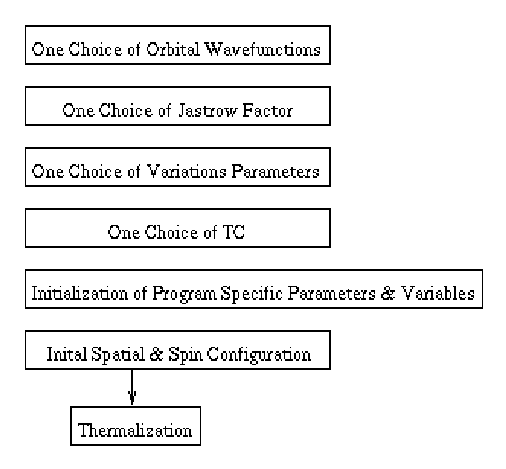
\epsfig{file=Implementation/initial_setup.eps, height=7.5cm}
  \caption{Initial setup}
  \label{initial_setup}
\end{center}
\end{figure}

In addition to the choice of trial wave-function, variational
parameters and TC, the program must initialize several parameters and
variables\footnote{These issues will be addressed {\bf
    \emph{later}}. }. Also, initial spatial coordinates of each
particle, and their respective spin, must be set.

The metropolis algorithm, {\bf \emph{described in
    section \ref{metropolis} }}, duplicates the behavior of the
wave-function. Before we begin the VMC sample, we want to make sure
that the particles initial positions are representative with respect
to the wave-function. Therefore, the metropolis algorithm is applied
several times to randomly chosen spatial and spin coordinates; the
coordinates are \emph{thermalized}.


%%%%%%%%%%%%%%%%%%%%%%%%%%%%%% VMC %%%%%%%%%%%%%%%%%%%%%%%%%%%%%%%%
\subsection{VMC}

Figure \ref{vmc} illustrates the basic principles of the different VMC
algorithms; all of which we wish to study in this thesis. 


\begin{figure}[hbtp]
\begin{center}
 % \epsfig{file=Implementation/vmc.eps, height=8.8cm}
  \input{Implementation/vmc.eepicemu}
  \caption{Three different algorithms for VMC: \newline
  (a) Move all/none particles \newline
  (b) Move one/no particle \newline
  (c) Move some particles}
  \label{vmc}
\end{center}
\end{figure}

In the first algorithm, figure \ref{vmc} (a), either all, or none, of
the particles are moved. This algorithm is easy to implement, but is
the most time-consuming of the three\footnote{Even though it is easy
  to implement, we will optimize our program with respect to the other
  two VMC algorithms. So, this ease is not reflexted in the code
  presented in \emph{?????}.}. In the second algorithm, depicted 
in figure \ref{vmc} (b), we sample the local energy after only one/no
particle is moved. In figure \ref{vmc} (c) we move some particles; 
we move one particle at a time, and conduct induvidual metropolis tests,
before we updating the local energy.

The \emph{Propose move} algorithm is depicted in figure \ref{propose_move}.

\begin{figure}[hbtp]
\begin{center}
  \epsfig{file=Implementation/propose_move.eps, height=3.8cm}
  \caption{Structure of \emph{Propose move}; proposed displacement of
    one particle}
  \label{propose_move}
\end{center}
\end{figure}

The \emph{Spin Flip} algorithm means that the particle may undergo a
spin flip with a randomly chosen particle. If the two particle have
the same spin, nothing happens. If the two particles have
different spin, the spins are exchanged. \newline
Two possible approches for the \emph{Randomize Position} algoritm:

\begin{enumerate}
  \item{}
    Variate position around the particles current location:

    \begin{equation*}
      x_{new}=x_{old}+\text{\small{RANDOM}}
    \end{equation*}

    where RANDOM is a random number based on e.g. a uniform distribution
    or a gaussian distribution.
  \item{}
    Importance Sampling:

    \begin{equation*}
      x_{new}=\Upsilon(\text{\small{RANDOM}})
    \end{equation*}

    where the function $\Upsilon$ duplicate the behaviour of the
    wave-function.
\end{enumerate}




%%%%%%%%%%%%%%%%%%%%%%%%%%%%%%%%%%%%%%%%%%%%%%%%%%%%%%%%%%%%%%%%%%%%%%
%                                                                    %
%                           Data Structure                           %
%                                                                    %
%%%%%%%%%%%%%%%%%%%%%%%%%%%%%%%%%%%%%%%%%%%%%%%%%%%%%%%%%%%%%%%%%%%%%%

\section{Data Structure}

We keep the Slater determinant and correlation wave-function in
separate classes. Let us start out with the correlation. For the
Metropolis step we need the ratio between the new and the old
wave-functions. Furthermore, we need the value of the correlation, and
its first and second derivatives, in order to preform a sample of the
local energy. \newline
We limit our attention to correlations, $G$ equal either $J$ or $e^J$,
where the Jastrow-factor is given by: 

\begin{equation}
  J = \sum_{i=0}^{\bar{N}}\sum_{j > i} f_{ij}
\end{equation}

where $N$ is the number of particles, $\bar{N}=N-1$, and

\begin{equation}
  f_{ij} = f(r_{ij})
\end{equation}

where $r_{ij}$ is the inter-electronic distance between electron $i$
and electron $j$.

Before we give the structure of the correlation, we first establish
classes to keep track of the inter-electronic distances,
\emph{Distance} and \emph{DistanceDiff}, the values of the $f_{ij}$'s,
\emph{Jastrow} and \emph{JastrowDiff}, and the derivatives,
\emph{Derivatives}.




%%%%%%%%%%%%%%%%%%%%% Distance and DistanceDiff %%%%%%%%%%%%%%%%%%%%
\subsection{Distance and DistanceDiff} 

The two classes, \emph{Distance} and \emph{DistanceDiff}, keep track
of the inter-electronic distances.  \newline
For \emph{Distance}, $r_{ij}$ is given by:

\begin{equation}
  r_{ij} = \left[
  \begin{array}{ccccccccc}
    0&r_{01}&r_{02}&\dots & r_{0i} &\dots &\dots & r_{0 \bar{N}} \\
    0&  0   &r_{12}&\dots & r_{1i} &\dots &\dots & r_{1 \bar{N}} \\
    0&  0   &  0   &\ddots& \vdots &\dots &\dots & \vdots       \\
    0&  0   &  0   &0& r_{\bar{i}i}&\dots &\dots & \vdots       \\
    0&  0   &  0   &  0   &  0&r_{ii^{^+}}&\dots & r_{i \bar{N}} \\
    0&  0   &  0   &  0   &   0    &  0   &\ddots& \vdots \\
    0&  0   &  0   &  0   &   0    &  0   & 0    &r_{\bar{\bar{N}} \bar{N}} \\
    0&  0   &  0   &  0   &   0    &  0   & 0    &  0
  \end{array} \right]
\label{r_ij}
\end{equation}

where $\bar{i}=i-1$, $i^{^+}=i+1$, $\bar{N}=N-1$ and
$\bar{\bar{N}}=N-2$. This information is stored in a single array of
length $N\dot(N-1)/2$, 

\begin{equation}
  \begin{array}{ccccc}
  rij =
  &|\underbrace{r_{01}, r_{02}, \dots, r_{0 \bar{N}} }
  &|\underbrace{ r_{12}, \dots, r_{1 \bar{N}} }
  &| \dots &|\underbrace{ r_{\bar{\bar{N}} \bar{N}} }  >\\
  & N-1 & N-2 & & 1\phantom{ii}
  \end{array}
  \label{r_ij_array}
\end{equation}

With a proposed move of electron $i$, only $N-1$ values need to be
updated. These values are stored in 

\begin{equation}
  rij\_new\_column = | r_{0i}, r_{1i}, \dots, r_{\bar{i}i}, r_{ii^{^+}},
  \dots, r_{i \bar{N}} >
\end{equation}

If the move is accepted, the values of \emph{rij\_new\_column} replace the
corresponding values in $rij$.

\emph{Distance} and
\emph{DistanceDiff} are quite similar, except \emph{DistanceDiff}
allows a variation of a coordinate.
For the \emph{DistanceDiff} class, the upper triangular matrix $r_{ij}$
is

\begin{equation}
  r_{ij} = \left[
  \begin{array}{ccccc}
    0 & r_{01}(\xi_1+h) & r_{02}(\xi_2+h)&\dots & r_{0 \bar{N}}(\xi_{\bar{N}}+h) \\
    0 &        0        & r_{12}(\xi_2+h)&\dots & r_{1 \bar{N}}(\xi_{\bar{N}}+h) \\
    0 &        0        &          0            &\ddots &  \vdots       \\
    0 &        0        &          0            &   0   &r_{\bar{\bar{N}} \bar{N}}(\xi_{\bar{N}}+h) \\
    0 &        0        &          0            &   0   &   0  
  \end{array} \right]
\label{r_ij_Diff}
\end{equation}

where $\xi$ is one of the cartesian coordinates. 

\begin{figure}[hbtp]
\begin{center}
  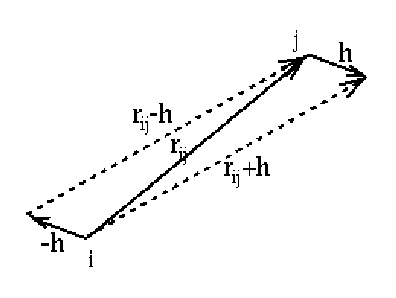
\epsfig{file=Implementation/vector_variation.eps, height=4cm}
  \caption{Addition of a vector at j equals the subtraction of the
  same vector at i}
  \label{vector_variation}
\end{center}
\end{figure}

As be can seen from figure \ref{vector_variation}\footnote{This is
  also easy to see from the relation $r_{ij} = \sqrt{
    \sum_{k=0}^{\bar{d}}(\xi_i^k-\xi_j^k)^2}$, 
where d is the number of dimensions, and $\bar{d}=d-1$.}, 

\begin{equation}
  r_{ij}(\xi_j+h) = r_{ij}(\xi_i-h)
\end{equation}

One object of class \emph{Distance} and 2d objects of class
\emph{DistanceDiff} holds all the information needed of the
inter-electronic distances for numerical calculation of both the
(centered difference) derivative and second derivative. Movement of
one electron consists of $(2d+1)\dot(N-1)$ updates of the distances,
and is thus of order ${\cal O}(N)$. Table \ref{Distance} give a list of the
public algorithms for the classes \emph{Distance} and
\emph{DistanceDiff}.

\begin{table}[hbtp]
\begin{center} {\large \bf Distance and DistanceDiff} \\ 
$\phantom{a}$ \\
\begin{tabular}{ll}
\hline\\ 
{\bf Algorithm}              & {\bf Usage} \\
Distance() or DistanceDiff() &Constructor\\
void attach(...)             &Attach intrinsic properties\\
void initialize()            &Initialize distances\\
void updateProposedMove()    &Calculate new distances for proposed move\\
void acceptMove()            &Accept proposed move\\
void rejectMove()            &Reject proposed move\\
double* getMatrix()          &Returns pointer to $rij$\\
double* getNewColumn()       &Returns pointer to $rij\_new\_column$\\
\hline
\end{tabular} 
\end{center}
\caption{Public algorithms for the classes Distance and DistanceDiff}
\label{Distance}
\end{table}

The differential parameters of
\emph{DistanceDiff}, $h$ and \emph{differentiate}, are assigned to
\emph{DistanceDiff} through the \emph{attach} algorithm. The value $h$
is the value added, or subtracted, to coordinate $differentiate$ of the
trial coordinate. \newline
An example on how to deal with upper triangular matrixes 
is in order. In the \emph{acceptMove} algorithm the new distances of
\emph{rij\_new\_column} is to be put into the upper-triangular matrix
$rij$. Here followes the \emph{acceptMove} algorithm:

{\footnotesize
\begin{enumerate}
\item[]
\begin{verbatim}
void Distance::acceptMove()
{
  __rij = rij-1+currentParticle;
  __rij_new_column = rij_new_column-1;
  int k=numParticles-1;
  for ( int i=0; i<currentParticle; i++ ) {
    (*__rij) = (*++__rij_new_column);
    k--;
    __rij+=k;
  }
  for ( int i=currentParticle+1; i<numParticles; i++)  
    (*++__rij)=(*++__rij_new_column);
  nextParticle();
}
\end{verbatim}

\end{enumerate}
}

For short we set $C=currentParticle$.
The pointer $\_\_rij$ is set to point at $r_{0C}$, if $C\ne
0$\footnote{If $C=0$ $\_\_rij$ is set to point at the element prior
  to the first element of $rij$},  
and $\_\_rij\_new\_column$ is set to point at the element
prior to the first element of $rij\_new\_column$\footnote{We
  create an extra element for this specific purpose.}.
Then we loop $i=0,C-1$, and set the value of $\_\_rij$ equal to the value
of the incremented $\_\_rij\_new\_column$, i.e. $r_{0C}$. We proceed
until $r_{\bar{C}C}$ (where $\bar{C}=C-1$). The pointer
$\_\_rij$ now points at $r_{\bar{C}\bar{N}}$, and in the
second loop it is incremented to point at $r_{CC^{^+}}$ (where $C^{^+}=C+1$),
and so is $\_\_rij\_new\_column$. Both pointers are incremented until
all the values are set, and we finally jump to the next particle.
\newline
Let us give an example of the $\_\_rij\_new\_column$ pointer. For $N=5$
and $C=2$ we have

\begin{equation}
  \begin{array}{cccccc}
  rij =
  |r_{01}, &r_{02}, \phantom{A} r_{03}, \phantom{A} r_{04}, &r_{12},
  \phantom{A} r_{13}, &r_{14}, &r_{23},
  &r_{24}, \phantom{A} r_{34}> \\
  pointer& \Uparrow \phantom{AAAAAAA}& \Uparrow \phantom{AAA}& \uparrow &
  \Uparrow & \Uparrow \phantom{AAAA}\\
  k& \phantom{AAA}3 & \phantom{AAAA}2 & \phantom{aa}1 & \phantom{aa}1 & 
  \end{array}
  \label{r_ij_array}
\end{equation}

We assign values at $\Uparrow$, and the $\uparrow$ is a temporary
pointer between the two loops.
This can more readily be seen by
looking at the corresponding matrix.

\begin{equation}
  r_{ij} = \left[
  \begin{array}{ccccc}
    0 & r_{01} & r_{02} & r_{03}  & r_{04}\\
    0 &   0    & r_{12} & r_{13}  & r_{14}\\
    0 &   0    &   0    & r_{23}  & r_{24}\\
    0 &   0    &   0    &   0     & r_{34}\\
    0 &   0    &   0    &   0     &   0   \\
  \end{array} \right]
\end{equation}

In the first loop we add one less than the number of none-zero
elements in the row we are at. Disregarding the none-zero elements,
this will take us to the element of the next row, with the same last index
(unless we are at the first element, in which case it will take us
to the last element).





%%%%%%%%%%%%%%%%%%%%% Jastrow and JastrowDiff %%%%%%%%%%%%%%%%%%%%
\subsection{Jastrow and JastrowDiff}

The classes \emph{Jastrow} and \emph{JastrowDiff} are similar to
\emph{Distance} and \emph{DistanceDiff}, respectively. First, they
contain information about the $f_{ij}$, in $f\_matrix$ (and the new
values for a proposed move, in \emph{f\_new\_column}). 
Furthermore, \emph{Jastrow} contains information about
the \emph{jastrowian}, $J$, and $\Delta J=J_{new}-J_{old}$.
Updating the $f_{ij}$'s for the jastrowian and its first and second
derivatives is also of order ${cal O}(N)$ (for the movement of one
electron).
Table \ref{Jastrow} lists the public algorithms of \emph{Jastrow} and
\emph{JastrowDiff}.

\begin{table}[hbtp]
\begin{center} {\large \bf Jastrow and JastrowDiff} \\ 
$\phantom{a}$ \\
\begin{tabular}{ll}
\hline\\ 
{\bf Algorithm}                        & {\bf Usage} \\
Jastrow() or JastrowDiff()             &  Constructor\\
void attach(...)                       &  Attach intrinsic properties\\
void initialize()                      &  Initialize the $f_{ij}$'s (and the jastrowian)\\
void updateProposedMove()              &Calculate new $f_{ij}$'s for proposed move\\
void acceptMove()                      &Accept proposed move\\
void rejectMove()                      &Reject proposed move\\
double* getFMatrix()                   &Returns pointer to $f\_matrix$\\
double* getFNewColumn()                &Returns pointer to $f\_new\_column$\\
void getFColumn(int i, double* fColumn)&Returns column i of $f\_matrix$ in fColumn\\
{\bf Jastrow-specific algorithms}      &\\
double\& operator()()                  &Returns the jastrowian, $J$\\
double getDifference()                 &Returns the difference, $\Delta J=J_{new}-J_{old}$\\
\hline
\end{tabular} 
 \end{center}
  \caption{Public algorithms for the classes Jastrow and JastrowDiff}
\label{Jastrow}
\end{table}

For example \emph{getFNewColumn} returns a pointer to:

\begin{equation}
  f\_new\_column = | f_{0i}, f_{1i}, \dots, f_{\bar{i}i}, f_{ii^{^+}},
  \dots, f_{i \bar{N}} >
\end{equation}

where $i$ is the current particle being moved.





%%%%%%%%%%%%%%%%%%%%% Derivatives %%%%%%%%%%%%%%%%%%%%
\subsection{Derivatives}

\emph{Derivatives} manages the derivatives of the $f_{ij}$'s. 
\newline
It is sufficient to calculate either $\frac{\delta f_{ij}}{\delta
  \xi_i}$ or $\frac{\delta f_{ij}}{\delta \xi_j}$, since 

\begin{equation}
  \frac{\delta f_{ij}}{\delta \xi_i} = \frac{\delta r_{ij}}{\delta \xi_i}
  \frac{d f_{ij}} {d r_{ij}} = - \frac{\delta r_{ij}}{\delta \xi_j}
  \frac{d f_{ij}} {d r_{ij}} = - \frac{\delta f_{ij}}{\delta \xi_j}
\end{equation}

In the above calculation we have used

\begin{equation}
  \frac{\delta r_{ij}}{\delta \xi_i^m} = \frac{\delta}{\delta \xi_i^m} 
  \sqrt{ \sum_{k=0}^{\bar{d}} (\xi_i^k-\xi_j^k)^2} =
  \frac{\xi_i^m-\xi_j^m}{r_{ij}} = - \frac{\delta
  r_{ij}}{\delta \xi_j^m} 
\end{equation}

where $\xi_i^m$ is cordinate $m$ of particle $i$, and $\bar{d}=d-1$. \newline
The upper triangular matrix:

\begin{equation}
  \frac{\delta f}{\delta \xi} = \left[
  \begin{array}{ccccc}
    0 & \frac{\delta f_{01}}{\delta \xi_1} & \frac{\delta
    f_{02}}{\delta \xi_2} & \dots & \frac{\delta f_{0\bar{N}}}{\delta
    \xi_{\bar{N}}} \\ 
    0 &        0        & \frac{\delta f_{12}}{\delta \xi_2} & \dots & 
    \frac{\delta f_{1\bar{N}}}{\delta \xi_{\bar{N}}} \\
    0 &        0        &          0            &\ddots &  \vdots       \\
    0 &        0        &          0            &   0   &
    \frac{\delta f_{\bar{\bar{N}}\bar{N}}}{\delta \xi_{\bar{N}}} \\
    0 &        0        &          0            &   0   &   0  
  \end{array} \right]
\label{df_dxi}
\end{equation}

is stored as an array, \emph{derivatives}, similar to that of
eq. (\ref{r_ij_array}). Also, we store 
the upper-triangular matrix of the second derivatives. The calculation
of the first derivative,

\begin{equation}
  \frac{\delta f_{ij}}{\delta \xi_i} \approx \frac{f_{ij}(\xi_i+h) -
  f_{ij}(\xi_i-h)}{2h} 
\end{equation}

and the second derivative,

\begin{equation}
  \frac{\delta^2 f_{ij}}{\delta \xi_i^2} \approx \frac{f_{ij}(\xi_i+h)
  + f_{ij}(\xi_i-h) - 2 f_{ij}}{h^2}
\end{equation}

uses the $f_{ij}$'s updated in \emph{Jastrow} and
\emph{JastrowDiff}. Movement of one particle involves
calculation of $N-1$ values of both $\frac{\delta f_{ij}}{\delta \xi_i}$
and $\frac{\delta^2 f_{ij}}{\delta \xi_i^2}$. Table \ref{Derivatives}
lists the public algorithms of \emph{Derivatives}.

\begin{table}[hbtp]
\begin{center} {\large \bf Derivatives} \\ 
$\phantom{a}$ \\
\begin{tabular}{ll}
\hline\\ 
{\bf Algorithm}                   & {\bf Usage} \\
Derivatives()                     &Constructor\\
void attach(...)                  &Attach intrinsic properties\\
void initialize()                 &Initialize the derivatives\\
void updateDerivatives()          &Calculate the new derivatives for a move\\ 
void acceptDerivatives()          &Updates the 1. and 2. derivatives matrix\\
void rejectDerivatives()          &Jumps to next particle without doing
anything\\
void getDColumn(int i, double* Column) 
  &Returns column i of $\frac{\delta f}{\delta \xi}$ in Column\\
double* getDNewColumn() &Returns pointer to new derivatives\\
void getD2Column(int i, double* Column)
  &Returns column i of $\frac{\delta^2 f}{\delta \xi^2}$ in Column\\
double* getD2NewColumn()&Returns pointer to new second derivatives\\
\hline
\end{tabular} 
 \end{center}
  \caption{Public algorithms for the class Derivatives}
\label{Derivatives}
\end{table}



%%%%%%%%%%%%%%%%%%%%% Correlation %%%%%%%%%%%%%%%%%%%%
\subsection{Correlation}

Before we proceed with the class structure, some theory must be
established. Let us start with the ratio
$\frac{G_{new}}{G_{old}}$, for the Metropolis algorithm. For $G=J$ we
have 

\begin{equation}
  \frac{G_{new}}{G_{old}} = \frac{J_{old}+\Delta J}{J_{old}}
\end{equation}

and for $G=e^J$,

\begin{equation}
  \frac{G_{new}}{G_{old}} = e^{\Delta J}
\end{equation}

$\nabla^2 J$ given by, 

\begin{equation}
  \nabla^2 J = \sum_{i=0}^{\bar{N}} \nabla_i^2 J =
  \sum_{i=0}^{\bar{N}} \nabla_i^2 \sum_{k<l} f_{kl} = 
  \sum_{i=0}^{\bar{N}} \left[ \sum_{k<l} \delta_{li} \nabla_i^2 f_{kl}
  + \sum_{k<l} \delta_{ki} \nabla_i^2 f_{kl} \right]
\end{equation}

where $\nabla_i^2 f_{ij} = \sum_{k=0}^{\bar{d}} \frac{\delta^2
  f_{ij}}{(\delta \xi_i^k)^2}$, and $\delta_{li}$ is the
Kronecker-delta. We define

\begin{equation}
  \nabla_i^2 J \equiv \sum_{j=0}^{i-1} \nabla_i^2 f_{ij}  +
  \sum_{j=i+1}^{\bar{N}} \nabla_j^2 f_{ij}
\end{equation}

and get 

\begin{equation}
  \nabla^2 J = \sum_{i=0}^{\bar{N}} \left[ \sum_{j=0}^{i-1} \nabla_i^2 f_{ij}
  + \sum_{j=i+1}^{\bar{N}} \nabla_i^2 f_{ij} \right] =
  \sum_{i=0}^{\bar{N}} \nabla_i^2 J
\end{equation}

from the relation $\nabla_i^2 f_{ij} = \nabla_j^2 f_{ij}$. If we move
one particle, $C$, all values in $\nabla^2_C J$, and one of the values
in $\nabla^2_i J$, $i\ne C$, are changed;

\begin{equation}
  \nabla_i^2 J^{new} = \nabla_i^2 J^{old} + \nabla_i^2 f_{iC}^{new} - \nabla_i^2 f_{iC}^{old}
\end{equation}

for all $i\ne C$, and

\begin{equation}
  \nabla_C^2 J^{new} = \sum_{i \ne C} \nabla_i^2 f_{iC}^{new}
\end{equation}

By changing only these values, we have an algorithm of order ${\cal O}(N)$
for the update of $\nabla^2 J$. \newline
For $\nabla J$, we have

\begin{equation}
  \nabla J = \left| \frac{\delta J}{\delta \xi_0^0},
  \dots , \frac{\delta J}{\delta \xi_{\bar{d}}^0}, \dots,
  \frac{\delta J}{\delta \xi_0^{\bar{N}}}, \dots, \frac{\delta J}{\delta
  \xi_{\bar{d}}^{\bar{N}}} \right>
\end{equation}

where

\begin{equation}
  \frac{\delta J}{\delta \xi^i} = \frac{\delta}{\delta \xi^i}
  \sum_{k<l} f_{kl} = \sum_{j=0}^{i-1} \frac{\delta f_{ji}}{\delta
  \xi^i}  + \sum_{j=i+1}^{\bar{N}} \frac{\delta f_{ij}}{\delta \xi^i} 
  = \sum_{j=0}^{i-1} \frac{\delta f_{ji}}{\delta
  \xi^i}  - \sum_{j=i+1}^{\bar{N}} \frac{\delta f_{ij}}{\delta \xi^j}
\end{equation}

since $\frac{\delta f_{ij}}{\delta \xi^i} = - \frac{\delta
  f_{ij}}{\delta \xi^j}$. 
All the values of the derivatives are kept
in the $d$ objects of class \emph{Derivatives}, and its easy to
calculate the above expression. However, we wish to keep the order of
our correlation routines as low as possible, so we follow a procedure
similar to that of $\nabla^2 J$;

\begin{equation}
  \frac{\delta J^{new}}{\delta \xi^i} = \frac{\delta J^{old}}{\delta
  \xi^i} + \frac{\delta f_{ji}^{new}}{\delta \xi^i} - \frac{\delta
  f_{ji}^{old}}{\delta \xi^i} 
\end{equation} 

for $i<C$,

\begin{equation}
  \frac{\delta J^{new}}{\delta \xi^i} = \frac{\delta J^{old}}{\delta
  \xi^i} - \frac{\delta f_{ji}^{new}}{\delta \xi^j} + \frac{\delta
  f_{ji}^{old}}{\delta \xi^j} 
\end{equation} 

for $i>C$, and for $C$

\begin{equation}
  \frac{\delta J^{new}}{\delta \xi^C} 
  = \sum_{j=0}^{C-1} \frac{\delta f_{jC}^{new}}{\delta
  \xi^C}  - \sum_{j=C+1}^{\bar{N}} \frac{\delta f_{Cj}^{new}}{\delta \xi^j}
\end{equation}

For $G=J$ we can use the above relations directly. For $G=e^J$ a few
minor modifications must be made:

\begin{equation}
  \nabla e^J = \nabla J \dot e^J
\end{equation}

and

\begin{equation}
  \nabla^2 e^J = \nabla (\nabla J \dot e^J) = \left[ \nabla^2 J +
  (\nabla J)^2  \right] e^J
\end{equation}

I.e. $e^J$, $\nabla J$ and $\nabla^2 J$ holds all the information needed to
compute $\nabla e^J$ and $\nabla^2 e^J$. The above computations are
also of the order ${\cal O}(N)$. \newline


\emph{Correlation} is the class used by the VMC-algorithm to manage
all information 
about the correlation. It is used to calculate the gradient, and the
gradient squared, of the correlation. Also, the ratio
$\frac{G_{new}}{G_{old}}$ for a proposed move is calculated, as well
as the value of the correlation, $G$, itself. Routines for both
thermalization- and VMC-moves are implemented. \newline
Table \ref{Correlation} lists the public algorithms of \emph{Correlation}.

\begin{table}[hbtp]
\begin{center} {\large \bf Correlation} \\ 
$\phantom{a}$ \\
\begin{tabular}{ll}
\hline\\ 
{\bf Algorithm}                 & {\bf Usage} \\
Derivatives(Domain\& domain)    &Constructor\\
void proposeMove()              &Updates the values (in the Jastrow and
Distance objects)\\
 & needed to determine the ratio $\frac{G_{new}}{G_{old}}$\\
void initializeThermalizedMove()&Initializes the Jastrow and Distance objects\\
void acceptThermalizedMove()    &Updates the Jastrow and Distance objects\\
void rejectThermalizedMove()    &Jumps to next particle without doing anything\\
void initializeVMC()            &Initializes the JastrowDiff, DistanceDiff 
              and Derivatives\\ 
&objects, and initializes $\nabla G$ and $\nabla^2 G$\\
void acceptVMCMove()            &Update $\nabla G$ and $\nabla^2 G$,
and updates the Jastrow, JastrowDiff,\\
& Distance, DistanceDiff and Derivatives objects\\
void rejectVMCMove()            &Jumps to next particle without doing anything\\
double operator()()             &Returns the correlation, $G$,
i.e. either $J$ or $e^J$\\
double getRatio()               &Returns the ratio $\frac{G_{new}}{G_{old}}$\\
double* getGradient()           &Returns pointer to $\nabla G$\\
double getGrad2()               &Returns the value of $\nabla^2 G$\\
\hline
\end{tabular} 
 \end{center}
  \caption{Public algorithms for the class Correlation}
\label{Correlation}
\end{table}

The constructor uses the \emph{Domain} class to access information
about properties like the number of particles $N$, the number of
dimensions $d$, and all the coordinates. The \emph{proposeMove}
algorithm updates the changes in the jastrowian due to a proposed move
in the trial coordinate. Furthermore, it stores the
new inter-electronic distances, and the new $f_{ij}$'s in two arrays;
\emph{rij\_new\_column} in the object of class\emph{Distance} and
\emph{f\_new\_column} in the object of class \emph{Jastrow}. \newline 
If the move is accepted, the values of the differences must be
updated, as well as the derivatives and the gradients (for a VMC
move\footnote{In the case of thermalization, no
  sample of the energy is preformed, so no derivatives (or
  differences) are calculated.}). 
In the \emph{acceptVMCmove} algorithm, see table \ref{Correlation}, the
values of $\nabla J$ and $\nabla^2 J$ are calculated. $\nabla G$
and $\nabla^2 G$ are not calculated until the \emph{getGradient} and
\emph{getGrad2} routines.
Finally, all new values must be assigned to their respective
upper-triangular matrices, before we proceed to the next particle. 
\newline
If the move is not accepted, we simply proceed to the next particle,
without performing any changes.



%%%%%%%%%%%%%%%%%%%%% CoorExt %%%%%%%%%%%%%%%%%%%%
\subsection{CoorExt}

The class \emph{CoorExt}, defined in \emph{Coor.h}, manages the
particles coordinates. Table 
\ref{CoorExt} lists the public algorithms of \emph{CoorExt}. 

\begin{table}[hbtp]
\begin{center} {\large \bf CoorExt} \\ 
$\phantom{a}$ \\
\begin{tabular}{ll}
\hline\\ 
{\bf Algorithm}                   & {\bf Usage} \\
CoorExt()                         & Empty constructor\\
CoorExt(double* x, int \_len,     & Constructor\\
\phantom{a} int \_\_spin, double* \_ext)& \\
void attach(double* \_\_x, int \_len,& Attaches intrinsic properties\\
\phantom{a} int \_\_spin, double* \_ext)& \\
double\& operator()()             & Returns the current cartesian coordinate\\
double\& operator()(int num)      & Returns coordinate num\\
void operator++(int)              & Increments pointer to next cartesian coordinate\\
void resetPtr                     & Resets pointer to first cartesian coordinate\\
int getLen()                      & Returns the number of cartesian coordinates\\
double r()                        & Returns the distance form the nucleus\\
void calculateR()                 & Computes the distance to the nucleus\\
int\& spin()                      & Returns the electron eigen-spin\\
int flipSpin()                    & Returns negative multiple of spin\\
double param(int i)               & Returns the value of parmeter number i; ext[i]\\
\hline
\end{tabular} 
 \end{center}
  \caption{Public algorithms for the class CoorExt}
\label{CoorExt}
\end{table}

\emph{CoorExt} contains all the information needed of each electron;
its cartesian coordinates and its eigen-spin. Furthermore, it contains
a pointer to the variational parameters of the Slater determinant
orbital wave-functions. In this manner one orbital function may be
computed directly given one \emph{CoorExt} object.
Also, the electron distance from the origin is calculated, and it
allows a spin flip.



%%%%%%%%%%%%%%%%%%%%% FuncSetMultivar %%%%%%%%%%%%%%%%%%%%
\subsection{FuncSetMultivar}

The class \emph{FuncSetMultivar}, defined in \emph{Func.h}, manages a
set of functions and their 
derivatives. Each column in a Slater matrix is represented as one such
object. Table \ref{FuncSetMultivar} lists some\footnote{All the
  \emph{attach} procedures are left out, Furthermore, most of the
  algorithms are implemented twice; ($\dots$) means either with or
  without an input (\emph{Param\& \_coordinate}).} of the public algorithms
of \emph{FuncSetMultivar}.

\begin{table}[hbtp]
\begin{center} {\large \bf FuncSetMultivar} \\ 
$\phantom{a}$ \\
\begin{tabular}{ll}
\hline\\ 
{\bf Algorithm}                   & {\bf Usage} \\
FuncSetMultivar($\dots$)          & Constructor\\
void init($\dots$)                & Initialize intrinsic properties\\
void calcValueCenter($\dots$)     & Calculates the function values (given coordinate)\\
void calcValueSides($\dots$)      & Calculates the function values (given differentiated coordinate)\\

double valuePt()                  & Returns pointer to different calculated values\\
double diff()                     & Calculates the first derivatives\\
double diff(int v)                & Calculates the first derivatives
with respect to the\\
                                  & indexed variable (of all functions)\\
double ddiff()                    & Calculates the second derivatives\\
\hline
\end{tabular} 
 \end{center}
  \caption{Public algorithms for the class FuncSetMultivar}
\label{FuncSetMultivar}
\end{table}

In order to find the derivatives of the functions for a given
coordinate, \emph{calcValueCenter} and \emph{calcValueSides}
must be called prior to \emph{diff}. The second derivatives are
calculated with a call to the \emph{ddiff} algorithm.



%%%%%%%%%%%%%%%%%%%%% Functor %%%%%%%%%%%%%%%%%%%%
\subsection{Functor}

The template class \emph{Functor} defines a functor. 
We have chosen to use a functor-type object, to increase
flexibility, and have the ability to use more complex functions
later without changing too much code\footnote{This is good programming
  philosophy; we may want to improve the program at a later stage.}.
Table \ref{Functor} lists the public algorithm of \emph{Functor}.

\begin{table}[hbtp]
\begin{center} {\large \bf Functor} \\ 
$\phantom{a}$ \\
\begin{tabular}{ll}
\hline\\ 
{\bf Algorithm}                   & {\bf Usage} \\
Functor()                         & Empty constructor\\
Functor(Function\& \_function)    & Constructor\\
void attach(Function\& \_function)& Attaches a function\\
Return operator()(Param\& coor)   & Returns an object of type Return\\
\hline
\end{tabular} 
 \end{center}
  \caption{Public algorithms for the class Functor}
\label{Functor}
\end{table}


Given an argument 
\emph{Param} the functor returns \emph{Return}. Both \emph{Param} and
\emph{Return} are classes, e.g. \emph{double}, \emph{CoorExt} etc.
To give an example, we can create a functor with the call:

{\footnotesize
\begin{enumerate}
\item[]
  \begin{verbatim}
Functor<CoorExt, double>* function;
function = new Functor<CoorExt, double>();
\end{verbatim}

\end{enumerate}
}

We need some formula for calculating the return value of type
\emph{double}, given an object of class \emph{CoorExt}. If we first
define the function \emph{hydr1s} given by:

{\footnotesize
\begin{enumerate}
\item[]
  \begin{verbatim}
double hydr1s(CoorExt& coordinate) {
  return exp(- coordinate.param(0) * coordinate.r());
}
\end{verbatim}

\end{enumerate}
}

and then attach it to the \emph{Functor} object \emph{function}:

{\footnotesize
\begin{enumerate}
\item[]
  \begin{verbatim}
function[0].attach(hydr1s);
\end{verbatim}

\end{enumerate}
}

We may then calculate the value of the function with the call:

{\footnotesize
\begin{enumerate}
\item[]
  \begin{verbatim}
function_value = (function[0])(coordinate);
\end{verbatim}

\end{enumerate}
}

where \emph{coordinate} is an object of class \emph{CoorExt}. 



%%%%%%%%%%%%%%%%%%%%% Random %%%%%%%%%%%%%%%%%%%%
\subsection{Random}

The two classes \emph{Ran0} and \emph{Ran1}, in
\emph{Random.h}, defines the random generators used by the
Metropolis random movement. We want our electrons to move \emph{randomly}
in space, and at the same time we want to reduce the CPU-time of our
calculations. Therefore, the program should be tested with different
random generators. Table \ref{Random} lists the
public algorithms of the random generators.

\begin{table}[hbtp]
\begin{center} {\large \bf Random} \\ 
$\phantom{a}$ \\
\begin{tabular}{ll}
\hline\\ 
{\bf Algorithm}                   & {\bf Usage} \\
Ran0(long seed) or Ran1(long seed)& Constructor\\
double getNum(void)               & Returns double in the range (0,1]\\
\hline
\end{tabular} 
 \end{center}
  \caption{Public algorithms for the class Random}
\label{Random}
\end{table}

We will not get into the details of the random generators, and simply
refere to \emph{???reference here???}. However, of importance to the
user is the integral seed. This seed is changed with each call to
\emph{getNum}. Giving the same seed twice produces the exact same
number, and if called several times they will produce the same
sequences of numbers. To produce indepentent runs, the seed
must differ with each run\footnote{An other problem may also
  arise. Even with two different seeds, one of the sequences may by
  chance produce the other seed, and thereby produce the same sequence
following this number. This problem will not be addressed in this
scope, but note that this chance is extremely small, and given two
different starting positions, the Metropolis algorithm should not
become too biased even if this were to occur.}











































\clearpage

\documentclass[../main.tex]{subfiles}
 
\begin{document}

\chapter{Results}\label{sec: Results}

Natural units ($\hbar=c=e=m_e=1$) were used to obtain all the results listed in this chapter.

\section{Optimization}

Here we look at the effect that various optimizations had on the computation time of our program. The optimization to the simulation itself gave a total speed-up factor of $31.246$ for the tested system, while running the program in parallel on $4$ processors gave an additional speed-up factor of around $3.6$.

\subsection{Storing Reused Data and Optmizing Hermite Polynomials}

For the following optimization results we used a system of two particles in a two-dimensional double harmonic oscillator well as reference system. For the results in Table \ref{tab: OptimizationExpansion} we used $465$ basis functions. From the table we see that including the "-ffast-math" compiler flag gives a decent speed up, but the storing of the Slater related matrices and the efficient computation of Hermite polynomials are the most important optimizations in this case. We also see that the "-ffast-math" flag is much more important when we include the Hermite optimization described in Section \ref{sec:Optimizing Hermite}. In this case the storing of the relative distances and the Jastrow related matrices, provide seemingly no speed up. This makes sense since these optimizations scale well with the number of particles used, and therefore become important for large numbers of particles. In our case we only have two particles so the effect of these optimizations is negligible. The optimization of Hermite polynomial calculation obviously scales with the number of Hermite polynomials we need. The number of Hermite polynomials we need scales with the number of basis functions we use, and in our case we use $465$ basis functions, which means we need the first $30$ Hermite polynomials, each of which has to be calculated many times for various positions of particles. The efficiency gain from storing the Slater related matrices also scales with the number of basis functions. This is because these matrices store the single particle wave functions and their derivatives. These single particle wave functions are calculated by a loop over the number of basis functions, so if we avoid recalculating them unnecessarily, we reduce the number of basis function loops, which of course is more important if we use a lot of basis functions.

\begin{table}[!ht]
  \centering
  \begin{tabular}{ | c | c | c | c |}
    \hline
    Optmizations & Avg. Time [s] & Speed Up & Total Speed Up\\*
    \hline
    B & 122.173 & 1.000 & 1.000\\*
    \hline
    B F & 104.244 & 1.172 & 1.172\\*
    \hline
    B F D & 104.296 & 1.000 & 1.171\\*
    \hline
    B F D S & 16.8304 & 6.197 & 7.259\\*
    \hline
    B F D S J & 16.8524 & 0.999 & 7.250\\*
    \hline
    B F D S J H & 3.91007 & 4.310 & 31.246\\*
    \hline
    B D S J H & 30.7192 & 0.127 & 4.017\\*
    \hline
  \end{tabular}
  \caption{Optimization results for two particles in a two-dimensional double harmonic oscillator well. The number of basis functions used was $465$. The letter B stands for base i.e. the program before doing optimizations. The letter F is for using the "-ffast-math" compiler flag, D is for storing the distance matrix, S is for storing the Slater related matrices, J is for storing the Jastrow related matrices, and H is for optimal computation of Hermite polynomials. The "Avg. Time" column is the average time over five runs, the "Speed Up" column lists the speed up factor relative to the row above, and the "Total Speed Up" column lists the speed up factor relative to the first row. Optimizations D and J have seemingly no effect on the run-time, because they scale with the number of particles and we only use two particles in this case. The gain from using the F optimization is much greater when we also use the H optimization. This is apparent by comparing the first two rows with the last two rows. The S and H optimizations provide the most speed up for this system.}
  \label{tab: OptimizationExpansion}
\end{table}

%\begin{table}[!ht]
%  \centering
%  \begin{tabular}{ | c | c | c | c | c | c | c | c | c |}
%    \hline
%    Optmizations & Run 1 & Run 2 & Run 3 & Run 4 & Run 5 & Avg. & Speed Up & Total\\*
%    \hline
%    B & 122.074 & 122.730 & 122.223 & 122.006 & 121.834 & 122.173 & 1.000 & 1.000\\*
%    \hline
%    B F & 104.236 & 104.029 & 103.951 & 104.515 & 104.489 & 104.244 & 1.172 & 1.172\\*
%    \hline
%    B F D & 103.960 & 104.523 & 104.207 & 104.359 & 104.429 & 104.296 & 1.000 & 1.171\\*
%    \hline
%    B F D S & 16.8619 & 16.6298 & 16.9949 & 16.8100 & 16.8552 & 16.8304 & 6.197 & 7.259\\*
%    \hline
%    B F D S J & 16.8360 & 16.9138 & 17.0127 & 16.8403 & 16.6593 & 16.8524 & 0.999 & 7.250\\*
%    \hline
%    B F D S J H & 3.99471 & 3.87888 & 3.89648 & 3.74037 & 4.03992 & 3.91007 & 4.310 & 31.246\\*
%    \hline
%    B D S J H & 30.8744 & 30.7226 & 30.8116 & 30.7741 & 30.4132 & 30.7192 & 0.127 & 4.017\\*
%    \hline
%  \end{tabular}
%  \caption{}
%  \label{tab: OptimizationExpansion}
%\end{table}

In order to see that storing the distances and the Jastrow related matrices do actually contribute to the optimization, we will look at a different system. We now look at a system of $24$ particles in a two-dimensional double harmonic oscillator well. However, we now approximate the single particle wave functions with super positions of two harmonic oscillator functions, similarly to what was done in Chapter 5.1.3 and 5.2.3 of Ref. \cite{Jorgen}. This means that the number of Hermite calculations needed is significantly reduced, and the effect of storing the distances and the Jastrow related matrices should stand out due to the increased number of particles. Note that this way of calculating the single particle wave functions is not the focus of this thesis, but it has been implemented in order to compare the results of the two methods. In this case we use this method in order to simulate $24$ particles with reasonably short run times, as this method is generally faster especially for large number of particles. The benefit of storing the distances and the Jastrow related matrices should be similar for both methods, since the difference between them is how the single particle wave functions are calculated, and these single particle wave functions do not depend on the Jastrow factor or the distances between particles. The optimization results for this system are listed in Table \ref{tab: OptimizationSupPos}. As expected the importance of storing the distances and the Jastrow related matrices has gone up. The storing of distances provide a decent speed up, while the storing of the Jastrow related matrices is in this case the most important optimization. The storing of the Slater related matrices is not quite as important as it was in Table \ref{tab: OptimizationExpansion}, but it still provides a pretty good speed up. The effect of using the "-ffast-math" flag is much smaller in this case, and the effect of calculating Hermite polynomials is negligible. This method needs a lot less Hermite polynomial calculations, since there is no loop over basis functions when calculating the single particle wave functions. However, the number of Hermite polynomial calculations does scale with the number of particles, and the recursive method becomes slow for large numbers of particles, so for systems with even more particles the Hermite optimization should become significant for this method as well.

\begin{table}[!ht]
  \centering
  \begin{tabular}{| c | c | c | c |}
    \hline
    Optmizations & Avg. Time [s] & Speed Up & Total Speed Up\\*
    \hline
    B & 103.576 & 1.000 & 1.000\\*
    \hline
    B F & 101.766 & 1.018 & 1.018\\*
    \hline
    B F D & 92.2338 & 1.103 & 1.123\\*
    \hline
    B F D S & 54.7138 & 1.686 & 1.893\\*
    \hline
    B F D S J & 10.7135 & 5.107 & 9.668\\*
    \hline
    B F D S J H & 10.6977 & 1.001 & 9.682\\*
    \hline
    B D S J H & 10.8811 & 0.983 & 9.519\\*
    \hline
  \end{tabular}
  \caption{Optimization results for $24$ particles in a two-dimensional double harmonic oscillator well. The letter B stands for base i.e. the program before doing optimizations. The letter F is for using the "-ffast-math" compiler flag, D is for storing the distance matrix, S is for storing the Slater related matrices, J is for storing the Jastrow related matrices, and H is for optimal computation of Hermite polynomials. The "Avg. Time" column is the average time over five runs, the "Speed Up" column lists the speed up factor relative to the row above, and the "Total Speed Up" column lists the speed up factor relative to the first row. The single particle wave functions were approximated by a super position of two harmonic oscillator functions instead of the method regularly used in this thesis. The method used here involves less Hermite polynomial calculations, and as a result, optimizing the calculation of Hermite polynomials is less important. The benefit of optimizations D and J should be similar between the methods, and now that the number of particles is increased the effect of these optimizations is also increased compared to Table \ref{tab: OptimizationExpansion}. Optimazation D now provides a decent speed up, while optimization J provides the majority of the total speed up. Optimization S also provides a good speed up, but it is not as significant as it was in Table \ref{tab: OptimizationExpansion}.}
  \label{tab: OptimizationSupPos}
\end{table}

%\begin{table}[!ht]
%  \centering
%  \begin{tabular}{ | c | c | c | c | c | c | c | c | c |}
%    \hline
%    Optmizations & Run 1 & Run 2 & Run 3 & Run 4 & Run 5 & Avg. & Speed Up & Total\\*
%    \hline
%    B & 103.804 & 103.122 & 103.119 & 104.314 & 103.523 & 103.576 & 1.000 & 1.000\\*
%    \hline
%    B F & 101.842 & 100.080 & 99.9448 & 100.403 & 106.561 & 101.766 & 1.018 & 1.018\\*
%    \hline
%    B F D & 91.8727 & 91.5986 & 94.2381 & 91.8457 & 91.6137 & 92.2338 & 1.103 & 1.123\\*
%    \hline
%    B F D S & 54.4560 & 55.5666 & 54.3716 & 54.3464 & 54.8286 & 54.7138 & 1.686 & 1.893\\*
%    \hline
%    B F D S J & 10.6361 & 10.9981 & 10.6575 & 10.7927 & 10.4832 & 10.7135 & 5.107 & 9.668\\*
%    \hline
%    B F D S J H & 10.5354 & 10.7410 & 10.9612 & 10.7303 & 10.5204 & 10.6977 & 1.001 & 9.682\\*
%    \hline
%    B D S J H & 10.8578 & 10.8000 & 10.8382 & 10.8467 & 11.0629 & 10.8811 & 0.983 & 9.519\\*
%    \hline
%  \end{tabular}
%  \caption{}
%  \label{tab: OptimizationSupPos}
%\end{table}

\subsection{Parallelization}

As discussed in Section \ref{sec:Parallel}, the variational Monte Carlo (VMC) simulation can be parallelized without mid-simulation communication between the processors. Therefore we can expect near linear scaling, so doubling the number of processors should about halve the run time. In Table \ref{tab: Parallel1} we have listed average run times for a system of two particles in a two-dimensional double harmonic oscillator well, when using $1275$ basis functions and $1$, $2$ and $4$ processors. From the table we see that the speed up is close to what we expect, but not quite. 

\begin{table}[!ht]
  \centering
  \begin{tabular}{| c | c | c | c |}
    \hline
    Processors & Avg. Time [s] & Speed Up & Total Speed Up\\*
    \hline
    1 & 36.9145 & 1.0000 & 1.0000\\*
    \hline
    2 & 19.1713 & 1.9255 & 1.9255\\*
    \hline
    4 & 10.3109 & 1.8593 & 3.5801\\*
    \hline
  \end{tabular}
  \caption{Parallelization results for two particles in a two-dimensional double harmonic oscillator well. The number of basis functions used was $1275$. The "Avg. Time" column is the average time over five runs, the "Speed Up" column lists the speed up factor relative to the row above, and the "Total Speed Up" column lists the speed up factor relative to the first row. We see that doubling the number of processors gives a speed up factor close to $2$, but it is still somewhat off, especially when going from $2$ to $4$ processors.}
  \label{tab: Parallel1}
\end{table}

A possible reason for why the results in Table \ref{tab: Parallel1} were somewhat different than expected could be that the run times were so short that the parallel overhead\footnote{Parallel overhead is the amount of time required to coordinate parallel tasks, as opposed to doing useful work. This can include factors such as: start-up time, synchronizations, data communications, software overhead imposed by libraries, operating system, etc., and termination time.\cite{Blaise}} was responsible for a significant fraction of the run time. If this is the case, doing the same test for a system that requires more CPU time, should provide results closer to the near linear scaling we expect. We increase the number of particles to $4$, and the run times for this system are listed in Table \ref{tab: Parallel2}. We end up with run times which are about three times as long as for the previous system, and as expected the speed up from parallelization is indeed somewhat greater for this system than for the two-particle system.

\begin{table}[!ht]
  \centering
  \begin{tabular}{| c | c | c | c |}
    \hline
    Processors & Avg. Time [s] & Speed Up & Total Speed Up\\*
    \hline
    1 & 107.468 & 1.0000 & 1.0000\\*
    \hline
    2 & 55.4418 & 1.9384 & 1.9384\\*
    \hline
    4 & 29.4316 & 1.8838 & 3.6514\\*
    \hline
  \end{tabular}
  \caption{Parallelization results for $4$ particles in a two-dimensional double harmonic oscillator well. The number of basis functions used was $1275$. The "Avg. Time" column is the average time over five runs, the "Speed Up" column lists the speed up factor relative to the row above, and the "Total Speed Up" column lists the speed up factor relative to the first row. We see that doubling the number of processors gives a speed up factor close to $2$, and the speed up factor are closer to $2$ in this case than they were in Table \ref{tab: Parallel1}. This is likely due to the generally longer run times for this system compared to the two-particle system. Since the run time is longer, the overhead is a smaller percentage of the total run time, which means it has less of an effect on the speed up factors.}
  \label{tab: Parallel2}
\end{table}

\section{Single Harmonic Oscillator Well}

In this section we look at the energy and one-body density of systems of particles in a single harmonic oscillator potential well, both in two and three dimensions.

\subsection{Ground State Energies}\label{sec: SHO GSE}

Here we look at the ground state energies for systems with various $\omega$ and number of particles. The ground state energies are calculated with the single particle wave functions being approximated by expansion in a single harmonic oscillator basis, and also by using harmonic oscillator single particle wave functions directly. Since the wave functions we are trying to approximate and the basis functions we use are of the same type (single harmonic oscillator) we should expect the two methods to yield the exact same results using a small amount of basis functions, just as we saw for the non-interacting case in Section \ref{sec:testSHO}. It turns out that we do not get the exact same results for the interacting case, however the same results are achieved if the variational parameter $\alpha$ is kept constant at $\alpha = 1$, while the other variational parameter $\beta$ is varied as usual. This indicates that there is an $\alpha$ dependence in the coefficients used in the basis function expansion, which our method fails to include. This $\alpha$ dependence could be included by doing a Hartree-Fock calculation on the coefficients, and this would be the next step in improving the method, but has not been done in this thesis.

\subsubsection{Two Dimensions}

The ground state energies for the two-dimensional case are listed in Table \ref{tab: EnergiesSHO2D}. The energies $E_\textrm{coeff}$ are the results when the single particle wave functions are approximated by expansion in a single harmonic oscillator basis, while $E_\textrm{reg}$ are the results when using harmonic oscillator single particle wave functions directly. We see from the table that $E_\textrm{coeff}$ and $E_\textrm{reg}$ are similar, especially for small numbers of particles $N$, but they are not exactly equal. Some further calculations not included here, revealed that the exact same energies where achieved if $\alpha$ was held constant at $\alpha = 1$, and $\beta$ was treated as the only variational parameter. This indicates that there is an $\alpha$ dependence in the coefficients used in the basis function expansion, which is not included when creating the coefficients. The coefficients could be modified to include this $\alpha$ dependence by doing a Hartree-Fock calculation, and if this is done $E_\textrm{coeff}$ and $E_\textrm{reg}$ should be exactly equal. 

The results $E_\textrm{coeff}$ and $E_\textrm{reg}$ are also bench-marked against results from various other methods such as Coupled Cluster and Full Configuration Interaction, as well as other VMC results. From Ref.~\cite{Taut} we also have an analytical result for the ground state energy, $E=3$, for the two-body case with $\omega=1$. The results are reasonably consistent with the benchmarks for all calculated systems. Our $E_\textrm{reg}$ results and the $E_\textrm{ref}^\textrm{(a)}$ benchmarks use the same VMC method, and as such should give fairly similar results. However, the optimization of parameters is done using different methods, which can result in slightly different parameter values being used, which in turn can result in differences larger than the statistical error. If the parameters used were exactly the same there could still be differences due to different amount of Monte Carlo cycles used, but in that case the statistical error would cover the difference. Table \ref{tab: DMCEnergiesSHO2D} has additional benchmarks from using Diffusion Monte Carlo, which is an improved version of VMC. Expanding our program to include DMC calculation as well as using Hartree-Fock to improve the coefficients is a possibility for further work.

\begin{table}[!ht]
  \centering
  \begin{tabularx}{\textwidth}{@{}ccYYYYYY@{}}%{ c c c c c c c c }
    \hline
    \hline
    $N$ & $\omega$ & $E_\textrm{coeff}$ & $E_\textrm{reg}$ & $E_\textrm{ref}^\textrm{(a)}$ & $E_\textrm{ref}^\textrm{(b)}$ & $E_\textrm{ref}^\textrm{(c)}$ & $E_\textrm{ref}^\textrm{(d)}$ \\*
    \hline
    2  & 0.01 & 0.0754(3) & 0.0745(2) & 0.07406(5) & - & 0.0738 \{23\} & 0.07383505 \{19\} \\*
       & 0.10 & 0.4460(3) & 0.4428(2) & 0.44130(5) & - & 0.4408 \{23\} & 0.44079191 \{19\} \\*
       & 0.28 & 1.0283(3) & 1.0245(3) & 1.02215(5) & - & 1.0217 \{23\} & 1.0216441 \{19\} \\*
       & 0.50 & 1.6658(3) & 1.6614(4) & 1.66021(5) & - & 1.6599 \{23\} & 1.6597723 \{19\} \\*
       & 1.00 & 3.0034(4) & 2.9984(4) & 3.00030(5) & - & 3.0002 \{23\} & 3.0000001 \{19\} \vspace{2 mm}\\*
    
    6  & 0.10 & 3.602(3) & 3.565(2) & 3.5690(3) & 3.49991 \{18\} & 3.5805 \{22\} & 3.551776 \{9\} \\*
       & 0.28 & 7.658(3) & 7.609(2) & 7.6216(4) & 7.56972 \{18\} & 7.6254 \{22\} & 7.599579 \{6\}  \\*
       & 0.50 & 11.853(3) & 11.781(2) & 11.8103(4) & 11.76228 \{18\} & 11.8055 \{22\} & 11.785915 \{6\} \\*
       & 1.00 & 20.243(3) & 20.143(3) & 20.1902(4) & 20.14393 \{18\} & 20.1734 \{22\} & 20.160472 \{8\} \vspace{2 mm}\\*
    
    12 & 0.10 & 12.568(7) & 12.282(3) & 12.3162(5) & 12.22533 \{17\} & 12.3497 \{21\} & 12.850344 \{3\} \\*
       & 0.28 & 25.866(6) & 25.642(4) & 25.7015(6) & 25.61084 \{17\} & 25.7095 \{21\} & 26.482570 \{2\} \\*
       & 0.50 & 39.406(5) & 39.152(4) & 39.2343(6) & 39.13899 \{17\} & 39.2194 \{21\} & 39.922693 \{2\} \\*
       & 1.00 & 65.952(5) & 65.666(4) & 65.7905(7) & 65.68304 \{17\} & 65.7399 \{21\} & 66.076116 \{3\} \\*
    \hline
    \hline
  \end{tabularx}
  \caption{The table lists ground state energy results for various single harmonic oscillator systems in two dimensions, and corresponding benchmarks. $N$ is the number of particles and $\omega$ is the harmonic oscillator frequency. $E_\textrm{coeff}$ are the energies obtained when the single particle wave functions are approximated by expansion in a single harmonic oscillator basis. For this the number of basis functions used was $(N/2)(N/2+1)/2$. $E_\textrm{reg}$ are the energies obtained when using harmonic oscillator single particle wave functions directly. The benchmarks are from the following: (a) J. Høgberget \cite{Jorgen} (VMC), (b) S. Reimann \cite{Reimann} (Similarity Renormalization Group theory), (c): C. Hirth \cite{Hirth} (Coupled Cluster Singles and Doubles), (d): V. K. B. Olsen \cite{Olsen} (Full Configuration Interaction). The numbers in parenthesis are the statistical errors found using blocking. In the curly brackets are the numbers of shells used above the last filled shell to construct the basis for the corresponding methods \cite{Jorgen}.}
  \label{tab: EnergiesSHO2D}
\end{table}

\begin{table}[!ht]
  \centering
  \begin{tabular}{c c c c}
    \hline
    \hline
    $N$ & $\omega$ & $E_\textrm{ref}^\textrm{(a)}$ & $E_\textrm{ref}^\textrm{(b)}$ \\*
    \hline
    2 & 0.01 & - & 0.073839(2) \\*
      & 0.10 & - & 0.44079(1) \\*
      & 0.28 & - & 1.02164(1) \\*
      & 0.50 & 1.65975(2) & 1.65977(1) \\*
      & 1.00 & 3.00000(3) & 3.00000(3) \vspace{2 mm}\\*
      
    6 & 0.10 & - & 3.55385(5) \\*
      & 0.28 & 7.6001(1) & 7.60019(6) \\*
      & 0.50 & 11.7888(2) & 11.78484(6) \\*
      & 1.00 & 20.1597(2) & 20.15932(8) \vspace{2 mm}\\*
      
    12 & 0.10 & - & 12.26984(8) \\*
       & 0.28 & 25.6356(1) & 25.63577(9) \\*
       & 0.50 & 39.159(1) & 39.1596(1) \\*
       & 1.00 & 65.700(1) & 65.7001(1) \\*
    \hline
    \hline
  \end{tabular}
  \caption{The table lists additional benchmarks for Table \ref{tab: EnergiesSHO2D}. $N$ is the number of particles and $\omega$ is the harmonic oscillator frequency. The benchmarks are from the following: (a) M. L. Pedersen et al. \cite{QDotBenchmarks} (DMC), (b) J. Høgberget \cite{Jorgen} (DMC).}
  \label{tab: DMCEnergiesSHO2D}
\end{table}

\subsubsection{Three Dimensions}

For the three-dimensional case the ground state energy results are listed in Table \ref{tab: EnergiesSHO3D}. Here we only have one source of benchmarks, but with both VMC and DMC benchmarks. From the table we mainly see the same things as for the two-dimensional case. The results are reasonably consistent with the benchmarks and with each other. By looking at the two particle case we can see that in general the energy is larger in three dimensions than in two dimensions for the same system, but the difference is smaller for smaller $\omega$. For $E_\textrm{reg}$ and $\omega = 0.01$ the ratio is $0.0790/0.0745 \approx 1.0604$, while for $\omega = 1$ it is $3.7242/2.9984 \approx 1.2421$.

\begin{table}[!ht]
  \centering
  \begin{tabularx}{\textwidth}{@{}ccYYYY@{}}%{ c c c c c c c c }
    \hline
    \hline
    $N$ & $\omega$ & $E_\textrm{coeff}$ & $E_\textrm{reg}$ & $E_\textrm{ref}^\textrm{(a)}$ & $E_\textrm{ref}^\textrm{(b)}$ \\*
    \hline
    2 & 0.01 & 0.0800(2) & 0.0790(1) & 0.07939(3) & 0.079206(3) \\*
      & 0.10 & 0.5004(2) & 0.4993(3) & 0.50024(8) & 0.499997(3) \\*
      & 0.28 & 1.2006(2) & 1.1993(3) & 1.20173(5) & 1.201725(2) \\*
      & 0.50 & 1.9977(2) & 1.9963(3) & 2.00005(2) & 2.000000(2) \\*
      & 1.00 & 3.7257(3) & 3.7242(3) & 3.73032(8) & 3.730123(3) \vspace{2 mm}\\*
      
    8 & 0.10 & 5.726(2) & 5.699(2) & 5.7130(6) & 5.7028(1) \\*
      & 0.28 & 12.210(2) & 12.172(2) & 12.2040(8) & 12.1927(1) \\*
      & 0.50 & 18.979(2) & 18.921(2) & 18.9750(7) & 18.9611(1) \\*
      & 1.00 & 32.685(2) & 32.593(2) & 32.6842(8) & 32.6680(1) \\*
    \hline
    \hline
  \end{tabularx}
  \caption{The table lists ground state energy results for various single harmonic oscillator systems in three dimensions, and corresponding benchmarks. $N$ is the number of particles and $\omega$ is the harmonic oscillator frequency. $E_\textrm{coeff}$ are the energies obtained when the single particle wave functions are approximated by expansion in a single harmonic oscillator basis. For this the number of basis functions used was $(N/2)(N/2+1)(N/2+2)/6$. $E_\textrm{reg}$ are the energies obtained when using harmonic oscillator single particle wave functions directly. The benchmarks are from the following: (a) J. Høgberget \cite{Jorgen} (VMC), (b) J. Høgberget \cite{Jorgen} (DMC). The numbers in parenthesis are the statistical errors found using blocking.}
  \label{tab: EnergiesSHO3D}
\end{table}


\subsection{One-Body Densities}

The one-body densities show us how the particles are likely to be distributed in the system. The main thing we look at is how far away from the center of the well a particle is most likely to be. However, it is also of interest to look a what (in the two-dimensional case) $x$ and $y$ positions are most likely independent of each other. In the first case we take the actual sampled positions of the particles and find the distance from the center of the well. In the second case we look at only the $x$ positions by themselves, and only the $y$ positions by themselves. Since the single harmonic oscillator well is symmetric, the $x$ distribution and the $y$ distribution should ideally be the same. 

We know that the harmonic oscillator external potential has its minimum in the center, i.e. at $r=0$. However, we also know that the particles have a Coulomb repulsion pushing the away from each other. So instead of the particles clumping together in the center of the well, they would be pushed away from the center by each other. At the same time they are confined by the external potential which pushes them back towards the center. Therefore the particles' most likely positions should be where the force from the other particles and the force from the external potential cancel each other. We expect $r$ to be greater than zero, but also limited by the external potential. As the number of particles increases the force between the particles will increase, which will push the particles further out until the force from the external potential is large enough to counteract the increased Coulomb repulsion. We can see this from the right-hand side of Figure \ref{fig:SHO_density3D_2d}. From the figure we see that for all numbers of particles $N$ the distribution has a top at $r>0$, and as $N$ increases this top is pushed further and further to the right, to greater and greater $r$ values. 

The $N=12$ case also shows a small change in the shape of the distribution indicating that some particles are closer to the center while others are further out, which corresponds to the particles being on different energy levels. This can be seen more clearly when looking at the $x$ and $y$ positions separately in Figure \ref{fig:SHO_density2d}, or at the $x$ and $y$ positions as a mesh-grid as seen on the left-hand side of Figure \ref{fig:SHO_density3D_2d}. The individual $x$ and $y$ distributions are almost identical as expected for a symmetric harmonic oscillator well.

\begin{figure}
\centering
\begin{subfigure}{0.48\textwidth}
\includegraphics[width=\linewidth]{figures/densitySHO/density_SHO_N6_Omega1_2d}
\caption{$N=6$} \label{fig:SHO_N6_2d_a}
\end{subfigure}\hspace*{\fill}
\begin{subfigure}{0.48\textwidth}
\includegraphics[width=\linewidth]{figures/densitySHO/density_SHO_N12_Omega1_2d}
\caption{$N=12$} \label{fig:SHO_N12_2d_b}
\end{subfigure}

\medskip
\begin{subfigure}{0.48\textwidth}
\includegraphics[width=\linewidth]{figures/densitySHO/density_SHO_N6_Omega1_2d_x}
\caption{$N=6$} \label{fig:SHO_N6_2d_x_c}
\end{subfigure}\hspace*{\fill}
\begin{subfigure}{0.48\textwidth}
\includegraphics[width=\linewidth]{figures/densitySHO/density_SHO_N12_Omega1_2d_x}
\caption{$N=12$} \label{fig:SHO_N12_2d_x_d}
\end{subfigure}

\medskip
\begin{subfigure}{0.48\textwidth}
\includegraphics[width=\linewidth]{figures/densitySHO/density_SHO_N6_Omega1_2d_y}
\caption{$N=6$} \label{fig:SHO_N6_2d_y_e}
\end{subfigure}\hspace*{\fill}
\begin{subfigure}{0.48\textwidth}
\includegraphics[width=\linewidth]{figures/densitySHO/density_SHO_N12_Omega1_2d_y}
\caption{$N=12$} \label{fig:SHO_N12_2d_y_f}
\end{subfigure}

\caption{Figures \ref{fig:SHO_N6_2d_a} and \ref{fig:SHO_N12_2d_b} show the one-body densities of a two-dimensional single harmonic oscillator with $N$ particles and $\omega=1$. The other figures show the corresponding distributions of $x$ and $y$ positions individually. The $x$ and $y$ distributions are almost identical due to the harmonic oscillator potential being symmetric.} \label{fig:SHO_density2d}
\end{figure}


\begin{figure}
\centering
\begin{subfigure}{0.48\textwidth}
\includegraphics[width=\linewidth]{figures/densitySHO/density3D_SHO_N2_Omega1_2d}
\caption{$N=2$} \label{fig:SHO_density3D_N2_a}
\end{subfigure}\hspace*{\fill}
\begin{subfigure}{0.48\textwidth}
\includegraphics[width=\linewidth]{figures/densitySHO/density_SHO_N2_Omega1_2d}
\caption{$N=2$} \label{fig:SHO_density_N2_b}
\end{subfigure}

\medskip
\begin{subfigure}{0.48\textwidth}
\includegraphics[width=\linewidth]{figures/densitySHO/density3D_SHO_N6_Omega1_2d}
\caption{$N=6$} \label{fig:SHO_density3D_N6_c}
\end{subfigure}\hspace*{\fill}
\begin{subfigure}{0.48\textwidth}
\includegraphics[width=\linewidth]{figures/densitySHO/density_SHO_N6_Omega1_2d}
\caption{$N=6$} \label{fig:SHO_density_N6_d}
\end{subfigure}

\medskip
\begin{subfigure}{0.48\textwidth}
\includegraphics[width=\linewidth]{figures/densitySHO/density3D_SHO_N12_Omega1_2d}
\caption{$N=12$} \label{fig:SHO_density3D_N12_e}
\end{subfigure}\hspace*{\fill}
\begin{subfigure}{0.48\textwidth}
\includegraphics[width=\linewidth]{figures/densitySHO/density_SHO_N12_Omega1_2d}
\caption{$N=12$} \label{fig:SHO_density_N12_f}
\end{subfigure}

\caption{The right-hand side shows the one-body densities of a two-dimensional single harmonic oscillator with $N$ particles and $\omega=1$. The left-hand side shows the distribution of positions for a mesh-grid of the $x$ and $y$ positions. From the left-hand side we can clearly see that the particles are divided into more energy levels as $N$ increases.} \label{fig:SHO_density3D_2d}
\end{figure}


\section{Double Harmonic Oscillator Well}

In this section we look at systems of particles in a double harmonic oscillator potential well, where the distance between the center of each well and the barrier between the wells is $L_x = 1$. We look at energies and one-body densities in both two and three dimensions.

\subsection{Ground State Energies}

Unlike for the single harmonic oscillator well, for the double harmonic oscillator well we have no reason to expect the results we get when the single particle wave functions are approximated by expansion in a single harmonic oscillator basis ($E_\textrm{coeff}$), to be exactly equal to the result from using harmonic oscillator single particle wave functions directly ($E_\textrm{reg}$). This is because the basis functions are still single harmonic oscillator functions, but the single particle wave functions we are trying to approximate are for a double harmonic oscillator well, so they are not of the same type as the basis functions. Because of this we should also expect to need more basis functions to get good results. Of course the $\alpha$ dependence discussed in Section \ref{sec: SHO GSE} is still missing from the coefficients. We compare $E_\textrm{coeff}$ with $E_\textrm{reg}$, and see that they are reasonably consistent with each other provided we use enough basis functions when calculating $E_\textrm{coeff}$.

\subsubsection{Two Dimensions}

The ground state energies of systems with various numbers of particles $N$ and harmonic oscillator frequencies $\omega$ are listed in Table \ref{tab: EnergiesDHO2D}. In most cases we need more basis functions to get good results for the double harmonic oscillator well, than we did for the single well, which is to be expected since the basis functions are single well functions. From the table we see that with a reasonable amount of basis functions we can achieve consistency between $E_\textrm{coeff}$ and $E_\textrm{reg}$. Unlike for the single well, here we only have one benchmark to compare our results to. In order to compare with the benchmark we have used the same distance between the wells as was used for the benchmark, i.e. $R=2$ in the $x$-direction, which corresponds to $L_x = 1$ in our case. From the table we see that our results are fairly consistent with the benchmark, but just as for the single well case, there are some difference likely due to some difference in the variational parameters.

For $N=2$ and $N=12$ we can directly compare the results of Table \ref{tab: EnergiesDHO2D} with those from Table \ref{tab: EnergiesSHO2D}. We see that given the same number of particles and the same $\omega$ the double well results are always smaller than their single well counterparts. This is expected since the particles are split between two wells in the double well. For example let us look at the $N=2$, $\omega = 1$ case. If $L_x$ was equal to $0$ the wells would be on top of each other, which means we essentially would have a single well potential, and the energy for a interacting system would then be $E=3$. If on the other hand $L_x$ was approaching infinity, then (assuming one particle in each well) the system could be considered as two independent single wells with one particle and consequently no interaction, and the energy would then be $E=2$. So for our case with $L_x=1$ we should expect $2<E<3$, and indeed we get $E_\textrm{coeff}=2.326$. If we imagine the $12$ particle case with $L_x$ approaching infinity there would still be interaction in each well, since there would be $6$ particles in each. However, for $N=6$, $\omega=1$ in Table \ref{tab: EnergiesSHO2D}, we have that $E_\textrm{coeff}=20.243$, so for the double well with $12$ particles and $L_x \rightarrow \infty$ the energy would be $E \approx 2\times 20.243 = 40.486$. Again the $L_x=0$ case corresponds to a single well with $12$ particles and for that we have the result $E_\textrm{coeff}=65.952$ from Table \ref{tab: EnergiesSHO2D}. So for the double well with $N=12$, $\omega=1$ we should expect $40.486<E<65.952$, and indeed we get $E_\textrm{coeff}=55.165$.

One thing to note about this is that while the double well results are smaller than the single well results in all cases, the difference between the two becomes very small as $\omega$ decreases. If we look at the $N=2$, $\omega=0.01$ case we see that for the single well we have $E_\textrm{coeff}=0.0754$ while for the double well we have $E_\textrm{coeff}=0.0735$. The reason for this is that as $\omega$ decreases the barrier between the wells in the double well becomes smaller and smaller, due to the widening of the wells. When this happens the double well starts to look more and more like a single well (though with an extended bottom). This is shown in Figure \ref{fig:DW}.

\begin{table}[!ht]
  \centering
  \begin{tabular}{c c c c c c}
    \hline
    \hline
    $N$ & $\omega$ & Basis Functions & $E_\textrm{coeff}$ & $E_\textrm{reg}$ & $E_\textrm{ref}$ \\*
    \hline
    2 & 0.01 & 1 & 0.0735(3) & 0.0727(2) & - \\*
      & 0.10 & 1 & 0.4106(9) & 0.4018(7) & -  \\*
      & 0.28 & 6 & 0.860(1) & 0.866(2) & - \\*
      & 0.50 & 6 & 1.336(2) & 1.339(2) & - \\*
      & 1.00 & 15 & 2.326(2) & 2.321(2) & 2.3496(1) \vspace{2 mm}\\*
      
    4 & 0.10 & 3 & 1.5966(9) & 1.5886(7) & - \\*
      & 0.28 & 10 & 3.362(1) & 3.222(1) & - \\*
      & 0.50 & 55 & 4.958(2) & 4.831(2) & - \\*
      & 1.00 & 55 & 7.850(2) & 7.848(2) & - \vspace{2 mm}\\*
      
    12 & 0.10 & 21 & 12.106(6) & 12.034(6) & - \\*
       & 0.28 & 21 & 23.771(6) & 23.785(7) & - \\*
       & 0.50 & 36 & 34.945(5) & 34.945(6) & - \\*
       & 1.00 & 45 & 55.165(6) & 55.226(6) & - \\*
    \hline
    \hline
  \end{tabular}
  \caption{The table lists ground state energy results for various double harmonic oscillator systems in two dimensions, and corresponding benchmarks. $N$ is the number of particles and $\omega$ is the harmonic oscillator frequency. $E_\textrm{coeff}$ are the energies obtained when the single particle wave functions are approximated by expansion in a single harmonic oscillator basis. $E_\textrm{reg}$ are the energies obtained when using double harmonic oscillator single particle wave functions directly. The benchmark is from J. Høgberget \cite{Jorgen} (DMC). The numbers in parenthesis are the statistical errors found using blocking.}
  \label{tab: EnergiesDHO2D}
\end{table}

\begin{figure}[!ht]
\centering
\begin{subfigure}{0.48\textwidth}
\includegraphics[width=\linewidth]{figures/DW_omega01}
\caption{$\omega=0.1$} \label{fig:DW_01}
\end{subfigure}\hspace*{\fill}
\begin{subfigure}{0.48\textwidth}
\includegraphics[width=\linewidth]{figures/DW_omega1}
\caption{$\omega=1$} \label{fig:DW_1}
\end{subfigure}

\caption{The shape of a double well potential with centers at $x=\pm1$ and $y=0$, for $\omega=0.1$ and $\omega=1$ with constant axes so they can be compared. $V(x)$ is the potential in the $x$-direction (double well) and $V(y)$ in the $y$-direction (single well). We see that for lower $\omega$, $V(x)$ is more similar to $V(y)$, indicating that the double well potential becomes more similar to a single well potential as $\omega$ decreases.} \label{fig:DW}
\end{figure}

\subsubsection{Three Dimensions}

The ground state energies for the three-dimensional case are listed in Table \ref{tab: EnergiesDHO3D}. For the three-dimensional case we do not have any benchmarks to compare our results with. However, we can still compare the results with each other, and from the table we see that $E_\textrm{coeff}$ and $E_\textrm{reg}$ are reasonably consistent with each other. In general we need more basis function to achieve good results for $E_\textrm{coeff}$, than we did in two dimensions. We also see that the similarities between the single well and the double well we observed in the two-dimensional case when $\omega$ was small, is also present in the three-dimensional case. As expected the energy is also generally larger for the three-dimensional case than for the two-dimensional case.

\begin{table}[!ht]
  \centering
  \begin{tabular}{c c c c c}
    \hline
    \hline
    $N$ & $\omega$ & Basis Functions & $E_\textrm{coeff}$ & $E_\textrm{reg}$ \\*
    \hline
    2 & 0.01 & 1 & 0.0782(2) & 0.0779(2) \\*
      & 0.10 & 10 & 0.4639(4) & 0.4652(5) \\*
      & 0.28 & 10 & 1.0642(7) & 1.0711(9) \\*
      & 0.50 & 10 & 1.7324(8) & 1.738(1) \\*
      & 1.00 & 35 & 3.212(2) & 3.194(2) \vspace{2 mm}\\*
      
    4 & 0.10 & 10 & 1.640(1) & 1.642(1) \\*
      & 0.28 & 56 & 3.518(1) & 3.483(2) \\*
      & 0.50 & 56 & 5.3858(9) & 5.360(2) \\*
      & 1.00 & 56 & 9.153(2) & 9.106(2) \\*
    \hline
    \hline
  \end{tabular}
  \caption{The table lists ground state energy results for various double harmonic oscillator systems in three dimensions. $N$ is the number of particles and $\omega$ is the harmonic oscillator frequency. $E_\textrm{coeff}$ are the energies obtained when the single particle wave functions are approximated by expansion in a single harmonic oscillator basis. $E_\textrm{reg}$ are the energies obtained when using double harmonic oscillator single particle wave functions directly. The numbers in parenthesis are the statistical errors found using blocking.}
  \label{tab: EnergiesDHO3D}
\end{table}


\subsection{One-Body Densities}

We are interested in looking at how particles are distributed in a double harmonic oscillator well. Just as for the single well, the particles will push each other away from the center, but here we do not just have a center for each well, we have a center between them at the potential barrier. We have placed this center at $r=0$, and each well center is a distance $r=1$ away. Going forward we will refer to this center as the system center. If there was no interaction between particles we would expect the particles to gather at the bottom of each well where the external potential is smallest. Since we have a repulsive interaction between the particles we expect the particles to push each other away from the well centers, just as we saw for the single well. Unlike for the single well, the well centers and the system center do not overlap for the double well so the mean distance between particles and the system center should be greater than an equivalent single well system. By comparing Figure \ref{fig:DHO_N12_2d_b} and \ref{fig:SHO_N12_2d_b} we see that for $N=12$ the mean value of $r$ is greater for a double well than for a single well. Just as for the single well, we also see that when going from $4$ particles to $12$ particles the mean value of $r$ increases.

In addition if we look at all particles in one well as a group, then that group should push the particles in the other well away from the system center and vice versa. This can be seen clearly from Figure \ref{fig:DHO_density3D_a} and \ref{fig:DHO_density3D_b}. In Figure \ref{fig:DHO_density3D_a} we have $N=2$ and one particle in each well and in Figure \ref{fig:DHO_density3D_b} we have $N=4$ and two particles in each well. In both cases the distribution ends up with one top for each well, however for the $N=4$ case the gap between the tops is larger and the distribution at the system center is smaller (as seen from the graph behind the surface plot). This is because when $N=4$ we have two groups of two particles pushing each other away from the system center, while in the $N=2$ case each group only has one particle and consequently the force on one group from the other is smaller than in the $N=4$ case.

When we increase the number of particles to $12$ we see from Figure \ref{fig:DHO_density3D_c} and \ref{fig:DHO_density3D_d} that the distribution gets a more interesting shape. For a well with $6$ particles in the single well case we saw from Figure \ref{fig:SHO_density3D_N6_c} that the distribution got a volcano like shape. However, when we have a double well with $6$ particles in each well we see from Figure \ref{fig:DHO_density3D_d} that the interaction force from one well on the other causes the volcano like shape to change into three tops surrounding the well center. The three tops are positioned as far away from each other as they can, and between the tops the distribution is somewhat smaller, but still fairly large.

In Figure \ref{fig:DHO_density2d} we have plots of the $x$ distribution and $y$ distribution separately for $N=4$ and $N=12$. The single well was symmetric so the distributions were identical in that case, but for the double well, we have a double well potential in the $x$-direction and a single well potential in the $y$-direction. The $y$ distributions get the same shape as they did for half as many particles in a single well (since each well has $N/2$ particles). The $x$ distributions however, get new shapes which clearly show that we have two identical wells separated by a barrier at $x=0$.

\begin{figure}[!ht]
\centering
\begin{subfigure}{0.48\textwidth}
\includegraphics[width=\linewidth]{figures/densityDHO/density_DHO_N4_Omega1_2d}
\caption{$N=4$} \label{fig:DHO_N4_2d_a}
\end{subfigure}\hspace*{\fill}
\begin{subfigure}{0.48\textwidth}
\includegraphics[width=\linewidth]{figures/densityDHO/density_DHO_N12_Omega1_2d}
\caption{$N=12$} \label{fig:DHO_N12_2d_b}
\end{subfigure}

\medskip
\begin{subfigure}{0.48\textwidth}
\includegraphics[width=\linewidth]{figures/densityDHO/density_DHO_N4_Omega1_2d_x}
\caption{$N=4$} \label{fig:DHO_N4_2d_x_c}
\end{subfigure}\hspace*{\fill}
\begin{subfigure}{0.48\textwidth}
\includegraphics[width=\linewidth]{figures/densityDHO/density_DHO_N12_Omega1_2d_x}
\caption{$N=12$} \label{fig:DHO_N12_2d_x_d}
\end{subfigure}

\medskip
\begin{subfigure}{0.48\textwidth}
\includegraphics[width=\linewidth]{figures/densityDHO/density_DHO_N4_Omega1_2d_y}
\caption{$N=4$} \label{fig:DHO_N4_2d_y_e}
\end{subfigure}\hspace*{\fill}
\begin{subfigure}{0.48\textwidth}
\includegraphics[width=\linewidth]{figures/densityDHO/density_DHO_N12_Omega1_2d_y}
\caption{$N=12$} \label{fig:DHO_N12_2d_y_f}
\end{subfigure}

\caption{Figure \ref{fig:DHO_N4_2d_a} and \ref{fig:DHO_N12_2d_b} show the one-body densities of a two-dimensional double harmonic oscillator with with centers at $x=\pm1$ and $y=0$, $N$ particles and $\omega=1$. The other figures show the corresponding distributions of $x$ and $y$ positions individually. Unlike the single well, the double well is not symmetric, so the $x$ and $y$ distributions are not identical.} \label{fig:DHO_density2d}
\end{figure}



\begin{figure}[!ht]
\centering
\begin{subfigure}{0.48\textwidth}
\includegraphics[width=\linewidth]{figures/densityDHO/density3D_DHO_N2_Omega1_2d}
\caption{$N=2$} \label{fig:DHO_density3D_a}
\end{subfigure}\hspace*{\fill}
\begin{subfigure}{0.48\textwidth}
\includegraphics[width=\linewidth]{figures/densityDHO/density3D_DHO_N4_Omega1_2d}
\caption{$N=4$} \label{fig:DHO_density3D_b}
\end{subfigure}

\medskip
\begin{subfigure}{0.48\textwidth}
\includegraphics[width=\linewidth]{figures/densityDHO/density3D_DHO_N12_Omega1_2d}
\caption{$N=12$} \label{fig:DHO_density3D_c}
\end{subfigure}\hspace*{\fill}
\begin{subfigure}{0.48\textwidth}
\includegraphics[width=\linewidth]{figures/densityDHO/density3D_DHO_N12_Omega1_2d_v2}
\caption{$N=12$} \label{fig:DHO_density3D_d}
\end{subfigure}

\caption{The figures show the distributions of positions for a mesh-grid of the $x$ and $y$ positions for a double harmonic oscillator well with centers at $x=\pm1$ and $y=0$. The number of particles is $N$ and the harmonic oscillator frequency is $\omega=1$. For $N=2$ and $N=4$ the distribution is fairly similar to two independent single wells, but for $N=12$ we get a more exiting shape exclusive to the double well. Figure \ref{fig:DHO_density3D_c} and \ref{fig:DHO_density3D_d} are the same, but from different angles.} \label{fig:DHO_density3D}
\end{figure}



\section{Finite Square Well}

In this section we look systems of particles in a finite square well potential with a distance of $2$ between the center and each wall. The value of the potential is $0$ inside the well and $1$ elsewhere. We look at energies and one-body densities in both two and three dimensions.

\subsection{Ground State Energies}

For the finite square well potential we do not have single particle wave functions we can use directly, so we can only approximate the single particle wave functions by expansion in a single harmonic oscillator basis. We also do not have any benchmarks, so we cannot compare our results to anything. Furthermore, as explained in Section \ref{sec: SHO GSE}, there is an $\alpha$ dependence missing from our overlap coefficients which means the optimization of $\alpha$ will not be accurate. In the harmonic oscillator systems this was not a problem since we had single particle wave functions we could use directly, which we then could use to find optimal parameters and use those parameters for both $E_\textrm{coeff}$ with $E_\textrm{reg}$. Due to this not being a possibility for the finite square well, we will here leave $\alpha$ constant at $\alpha = 1$ and just vary $\beta$. Of course this will not guarantee that our results come close to the true ground states, but we can still use the results to get an idea of how many basis functions are needed for good results, and whether or not using harmonic oscillator basis functions is practical for a finite square well potential.

\subsubsection{Two Dimensions}

Ground state energy results for a two-dimensional finite square well with $N$ particles are listed in Table \ref{tab: EnergiesFSW2D}. The finite square well potential does not have a harmonic oscillator frequency $\omega$, however the harmonic oscillator basis functions we use still do. Because of this we should expect similar results regardless of the value of $\omega$ as long as we use a sufficient amount of basis functions. Still, what amount of basis functions that is sufficient will depend on $\omega$, since some $\omega$ values will yield basis functions which fit better with the finite square well than others. This is illustrated in Figure \ref{fig: FSW_omega_comp}. From the figure we see that the most fitting $\omega$ value would be somewhere between $\omega = 0.1$ and $\omega = 1$.

From Table \ref{tab: EnergiesFSW2D} we see that for $N=2$, both for $\omega = 0.1$ and $\omega = 1$, the energy converges as the number of basis functions becomes sufficient. The energy values we end up with are not exactly the same for both $\omega$ values, but they are reasonably close to each other. The discrepancy could be due to keeping $\alpha$ constant at $1$. From the table it also seems like the energy converges faster with increasing number of basis functions for $\omega = 0.1$ than for $\omega = 1$. However, the optimization of $\beta$ is also dependent on how many basis functions are used, and from Table \ref{tab: EnergiesFSW2D_v2} we see that if we use $120$ basis functions for optimizing $\beta$, but $15$ basis functions to do the actual calculation with the optimized $\beta$, then we get better results for $\omega = 1$ than for $\omega = 0.1$. So it would seem that with $\omega = 0.1$ we need fewer basis functions to find an optimal $\beta$, but given an optimal $\beta$ we need fewer basis functions to get good results with $\omega = 1$ than with $\omega = 0.1$.

Overall, it seems that for the finite square well we need more harmonic oscillator basis functions than we do for a double harmonic oscillator well, and as $N$ increases the amount of basis functions needed may be impractical computational cost wise. It may be better to use other types of basis functions, e.g. hydrogen-like wave functions. It would be a good idea though, to do a Hartree-Fock calculation on the overlap coefficients and then properly optimizing $\alpha$ as well as $\beta$, to see how many basis functions are needed in that case.


\begin{table}[!ht]
  \centering
  \begin{tabular}{c c c c c}
    \hline
    \hline
    $N$ & $\omega$ & Basis Functions & $E_\textrm{coeff}$ \\*
    \hline
    2 & 0.10 & 15 & 1.33(2) \\*
      & 0.10 & 45 & 1.271(5) \\*
      & 0.10 & 78 & 1.266(5) \\*
      & 0.10 & 120 & 1.265(5) \\*
      & 1.00 & 15 & 1.525(6) \\*
      & 1.00 & 45 & 1.450(5) \\*
      & 1.00 & 78 & 1.281(2) \\*
      & 1.00 & 120 & 1.281(2) \vspace{2 mm}\\*
      
    6 & 0.10 & 45 & 9.38(5) \\* %9.710(8) 0.5beta
      & 1.00 & 45 & 10.689(5) \\*
    \hline
    \hline
  \end{tabular}
  \caption{The table lists ground state energy results for various finite square well systems in two dimensions. $N$ is the number of particles. $E_\textrm{coeff}$ are the energies obtained when the single particle wave functions are approximated by expansion in a single harmonic oscillator basis, and $\omega$ is the harmonic oscillator frequency used for the harmonic oscillator basis functions. The numbers in parenthesis are the statistical errors found using blocking. For $N=2$ we see that the energies converge as long as enough basis functions are used, but the somewhat high number of basis functions needed may be impractical with regards to computational cost, especially for higher $N$.}
  \label{tab: EnergiesFSW2D}
\end{table}

\begin{table}[!ht]
  \centering
  \begin{tabular}{c c c c c}
    \hline
    \hline
    $N$ & $\omega$ & Basis Functions & $E_\textrm{coeff}$ \\*
    \hline
    2 & 0.10 & 15\{120\} & 1.32(2) \\*
      & 1.00 & 15\{120\} & 1.296(2) \\*
    \hline
    \hline
  \end{tabular}
  \caption{Additional results for Table \ref{tab: EnergiesFSW2D}. However, here the amount of basis functions used to optimize $\beta$ (curly brackets), and the amount of basis function used to do the actual energy calculation are not the same. Based on this table and Table \ref{tab: EnergiesFSW2D}, it would seem that for $\omega=0.1$ we need fewer basis functions to properly optimize $\beta$, but given an optimal $\beta$ value, we need fewer basis functions to get good results for $\omega = 1$ than for $\omega = 0.1$.}
  \label{tab: EnergiesFSW2D_v2}
\end{table}

\begin{figure}
\centering
\includegraphics[width=\linewidth]{figures/SW_omega_comp}
\caption{Comparison between the finite square well potential and harmonic oscillators with different $\omega$ values. From the figure we can see the effect $\omega$ has on how good a fit harmonic oscillator basis functions are to the finite square well potential. It appears that the optimal $\omega$ value would be somewhere between $\omega = 0.1$ and $\omega = 1$.}
\label{fig: FSW_omega_comp}
\end{figure}

\subsubsection{Three Dimensions}

For the three-dimensional case we see from Table \ref{tab: EnergiesFSW3D} that we need a lot more basis function for the energies to converge than we did for the two-dimensional case. As always we expect the energies to be greater for three-dimensions than for two-dimensions, and from the table we see that that holds true here as well.

\begin{table}[!ht]
  \centering
  \begin{tabular}{c c c c c}
    \hline
    \hline
    $N$ & $\omega$ & Basis Functions & $E_\textrm{coeff}$ \\*
    \hline
    2 & 0.10 & 165 & 1.412(5) \\*
      & 0.10 & 364 & 1.411(5) \\*
      & 1.00 & 165 & 1.465(3) \\*
      & 1.00 & 364 & 1.463(3) \\*
    \hline
    \hline
  \end{tabular}
  \caption{The table lists ground state energy results for various finite square well systems in three dimensions. $N$ is the number of particles. $E_\textrm{coeff}$ are the energies obtained when the single particle wave functions are approximated by expansion in a single harmonic oscillator basis, and $\omega$ is the harmonic oscillator frequency used for the harmonic oscillator basis functions. The numbers in parenthesis are the statistical errors found using blocking. The amount of basis functions needed for the energies to converge is a lot greater for three dimensions than for two.}
  \label{tab: EnergiesFSW3D}
\end{table}

\subsection{One-Body Densities}

For the specific finite square well we have looked at in this thesis we expect all particles to be within the well, so-called bound particles, if the number of particles $N$ is $6$ or less. For our well being inside the well corresponds to having $r<\sqrt{8}$. Since the walls are $x,y = 2$ away from the center, the furthest away from the center a particle should be is in one of the corners, i.e. the particle would have $x$ and $y$ positions close to $\pm 2$, which would give an $r$ value close to $\sqrt{2^2 + 2^2}$. So for the one-body density we expect the distribution of $r$ to be $0$ at $r>\sqrt{8}$. 

From Figure \ref{fig:FSW_N2_2d} we see that for $N=2$, $\omega = 0.1$ and $15$ basis functions the particles are not completely bound, but for $\omega = 1$ they are (mostly). However, as the number of basis functions increase the distribution for $\omega = 0.1$ converges towards a final shape quicker than for $\omega = 1$. This fits with the energy results, where we saw that for $\omega = 0.1$ we need more basis functions to get good results, but for $\omega = 0.1$ we also find the optimal $\beta$ value with fewer basis functions. The shape for $\omega = 0.1$ is worse with $15$ basis functions because, even with an optimal $\beta$, $\omega = 0.1$ yields bad results for that few basis functions. However, the shape for $\omega = 0.1$ improves quicker as the number of basis functions increases because the optimal $\beta$ is reached with fewer basis functions. From Figure \ref{fig:FSW_N6_2d} we see that for $N=6$ with $\omega = 0.1$, the issue from $N=2$ with $15$ basis functions occurs even if we use $45$ basis functions. This shows the need for more basis functions as the number of particles increases.

Unlike for harmonic oscillator potential, for the square well potential the strength of the potential is constant until we hit one of the walls, at which point the potential skyrockets. For $N=2$ we should then expect the most likely position of the particle to be one that minimizes the repulsive forces between them while still keeping both particles within the well. In order to achieve this the particles should be in corners diagonally opposite of each other. This would mean that the distribution of $r$ should have a top at $r \approx \sqrt{8}$ in the two-dimensional case. However, when we look at our distributions in Figure \ref{fig:FSW_N2_2d_b} we see that the top of the distributions are typically between $r=1$ and $r=2$. This is likely due to the fact that we keep $\alpha$ constant at $1$, and doing a Hartree-Fock calculation on the overlap coefficient and properly optimizing $\alpha$ should solve this issue. From Figure \ref{fig:FSW_density3D} we can see that for $N=6$ particles the distribution has tops in the four corners, which is expected since it suggests that it is most likely for there to be one particle in each corner, and the last two being somewhere in the middle.

\begin{figure}[!ht]
\centering
\includegraphics[width=\linewidth]{figures/densityFSW/density3D_FSW_N6_Omega1_2d_BF45}
\caption{The figures show the distributions of positions for a mesh-grid of the $x$ and $y$ positions for a finite square well potential. The number of particles is $N$ and the harmonic oscillator frequency used for the basis functions is $\omega=1$. We see that the distribution has tops at the corners of the well, which makes sense since the strength of the potential is equal everywhere inside the well and the Coulomb repulsion pushes the particles away from each other.} \label{fig:FSW_density3D}
\end{figure}

\begin{figure}
\centering
\begin{subfigure}{0.48\textwidth}
\includegraphics[width=\linewidth]{figures/densityFSW/density_FSW_N2_Omega010_2d_BF15.pdf}
\caption{$\omega=0.1$, $15$ Basis Functions} \label{fig:FSW_N2_2d_a}
\end{subfigure}\hspace*{\fill}
\begin{subfigure}{0.48\textwidth}
\includegraphics[width=\linewidth]{figures/densityFSW/density_FSW_N2_Omega1_2d_BF15.pdf}
\caption{$\omega=1$, $15$ Basis Functions} \label{fig:FSW_N2_2d_b}
\end{subfigure}

\medskip
\begin{subfigure}{0.48\textwidth}
\includegraphics[width=\linewidth]{figures/densityFSW/density_FSW_N2_Omega010_2d_BF45.pdf}
\caption{$\omega=0.1$, $45$ Basis Functions} \label{fig:FSW_N2_2d_c}
\end{subfigure}\hspace*{\fill}
\begin{subfigure}{0.48\textwidth}
\includegraphics[width=\linewidth]{figures/densityFSW/density_FSW_N2_Omega1_2d_BF45.pdf}
\caption{$\omega=1$, $45$ Basis Functions} \label{fig:FSW_N2_2d_d}
\end{subfigure}

\medskip
\begin{subfigure}{0.48\textwidth}
\includegraphics[width=\linewidth]{figures/densityFSW/density_FSW_N2_Omega010_2d_BF120.pdf}
\caption{$\omega=0.1$, $120$ Basis Functions} \label{fig:FSW_N2_2d_e}
\end{subfigure}\hspace*{\fill}
\begin{subfigure}{0.48\textwidth}
\includegraphics[width=\linewidth]{figures/densityFSW/density_FSW_N2_Omega1_2d_BF120.pdf}
\caption{$\omega=1$, $120$ Basis Functions} \label{fig:FSW_N2_2d_f}
\end{subfigure}

\caption{One-body densities for a two-dimensional finite square well potential with $N=2$ particles. The distance between the well center and each wall is $2$, and the potential is $0$ inside the well and $1$ outside.} \label{fig:FSW_N2_2d}
\end{figure}


\begin{figure}
\centering
\begin{subfigure}{0.48\textwidth}
\includegraphics[width=\linewidth]{figures/densityFSW/density_FSW_N6_Omega010_2d_BF45.pdf}
\caption{$\omega=0.1$, $45$ Basis Functions} \label{fig:FSW_N6_2d_a}
\end{subfigure}\hspace*{\fill}
\begin{subfigure}{0.48\textwidth}
\includegraphics[width=\linewidth]{figures/densityFSW/density_FSW_N6_Omega1_2d_BF45.pdf}
\caption{$\omega=1$, $45$ Basis Functions} \label{fig:FSW_N6_2d_b}
\end{subfigure}

\caption{One-body densities for a two-dimensional finite square well potential with $N=6$ particles. The distance between the well center and each wall is $2$, and the potential is $0$ inside the well and $1$ outside.} \label{fig:FSW_N6_2d}
\end{figure}


\begin{figure}
\centering
\begin{subfigure}{0.48\textwidth}
\includegraphics[width=\linewidth]{figures/densityFSW/density_FSW_N2_Omega010_3d_BF364.pdf}
\caption{$\omega=0.1$, $364$ Basis Functions} \label{fig:FSW_N2_3d_a}
\end{subfigure}\hspace*{\fill}
\begin{subfigure}{0.48\textwidth}
\includegraphics[width=\linewidth]{figures/densityFSW/density_FSW_N2_Omega1_3d_BF364.pdf}
\caption{$\omega=1$, $364$ Basis Functions} \label{fig:FSW_N2_3d_b}
\end{subfigure}

\caption{One-body densities for a three-dimensional finite square well potential with $N=2$ particles. The distance between the well center and each wall is $2$, and the potential is $0$ inside the well and $1$ outside.} \label{fig:FSW_N2_3d}
\end{figure}

\begin{comment}
\section{Wave Function Expanded in Harmonic Oscillator Basis}
\begin{table}[!ht]
  \centering
  \begin{tabular}{ | c | c | c | }
    \hline
    $N$ & $E$ (\textrm{Shared start}) & $E$ (\textrm{Split start}) \\*
    \hline
    $2$ & $2.00002$ & $2.00002$ \\*
    \hline
    $4$ & $4.00005$ & $4.00005$ \\*
    \hline
    $6$ & $8.00009$ & $8.0001$ \\*
    \hline
  \end{tabular}
  \caption{Unperturbed energies for the double well when approximating the single particle wave functions with harmonic oscillator basis functions. Results in the second column are for when all the particles starts in the same well and are then distributed between the wells by the program, while the results in the third column are for when we force half of the particles in each well at the start. Two dimensional system, $L_x=4$, $\omega=1$.}
  \label{tab: unperturbedEnergiesCoeff}
\end{table}

\begin{table}[!ht]
  \centering
  \begin{tabular}{ | c | c | c | }
    \hline
    $N$ & $E$ (\textrm{Shared start}) & $E$ (\textrm{Split start}) \\*
    \hline
    $2$ & $3.00854$ & $2.34952$ \\*
    \hline
    $4$ & $6.53324$ & $6.53747$ \\*
    \hline
    $6$ & $14.1804$ & $14.2108$ \\*
    \hline
  \end{tabular}
  \caption{Perturbed energies for the double well when approximating the single particle wave functions with harmonic oscillator basis functions. Results in the second column are for when all the particles starts in the same well and are then distributed between the wells by the program, while the results in the third column are for when we force half of the particles in each well at the start. Two dimensional system, $L_x=4$, $\omega=1$.}
  \label{tab: perturbedEnergiesCoeff}
\end{table}

\section{Wave Function as Super Postion of two Harmonic Oscillator Functions}
\begin{table}[!ht]
  \centering
  \begin{tabular}{ | c | c | c | }
    \hline
    $N$ & $E$ (\textrm{Shared start}) & $E$ (\textrm{Split start}) \\*
    \hline
    $2$ & $2$ & $2$ \\*
    \hline
    $4$ & $4$ & $4$ \\*
    \hline
    $6$ & $8$ & $8$ \\*
    \hline
  \end{tabular}
  \caption{Unperturbed energies for the double well when approximating the single particle wave functions with a super position of two harmonic oscillator functions. Results in the second column are for when all the particles starts in the same well and are then distributed between the wells by the program, while the results in the third column are for when we force half of the particles in each well at the start. Two dimensional system, $L_x=4$, $\omega=1$.}
  \label{tab: unperturbedEnergiesSupPos}
\end{table}

\begin{table}[!ht]
  \centering
  \begin{tabular}{ | c | c | c | }
    \hline
    $N$ & $E$ (\textrm{Shared start}) & $E$ (\textrm{Split start}) \\*
    \hline
    $2$ & $3.00852$ & $2.3495$ \\*
    \hline
    $4$ & $6.53322$ & $6.53742$ \\*
    \hline
    $6$ & $14.4748$ & $13.872$ \\*
    \hline
  \end{tabular}
  \caption{Perturbed energies for the double well when approximating the single particle wave functions with a super position of two harmonic oscillator functions. Results in the second column are for when all the particles starts in the same well and are then distributed between the wells by the program, while the results in the third column are for when we force half of the particles in each well at the start. Two dimensional system, $L_x=4$, $\omega=1$.}
  \label{tab: perturbedEnergiesSupPos}
\end{table}
\end{comment}

\end{document}
\clearpage

\chapter{Conclusion}\label{sec:conclusion}
\subsubsection{Concluding Points}

In conclusion, this thesis has explored the application of various machine learning techniques to solve quantum many-body problems, specifically focussing on one-dimensional trapped spinless fermions and two-dimensional quantum dots. By making use of neural networks such as Deep Set feed-forward networks (DSFFN) and restricted Boltzmann machines (RBM), we have demonstrated the potential of these networks to be used as variational Monte Carlo (VMC) functions, following ideas of reinforcement learning. From our findings, this approach enabled us to approximate ground-state energies and wavefunctions with good accuracy.

In particular, the effectiveness of neural network ansätze was evident as the DSFFN in combination to stochastic reconfiguration yielded in an isolated case, energy values below DMC calculations, and overall very good results. If an average analysis of the energies is made and if we disregard the stochastic reconfiguration method due to its difficult convergence behaviour, the RBM implementation was slightly favoured in the two-dimensional fermionic trap with Coulomb interaction. In contrast, for the one-dimensional case, where SR convergence was easy and used for all ansätze, the VMC without neural networks was optimal.

In general, the inclusion of correlation factors, such as the Jastrow and Padé-Jastrow factors, significantly improved the energy estimates, bringing them closer to the reference values of other research. This improvement from the addition of correlation factors was present in both one-dimensional and two-dimensional systems, and the Padé-Jastrow factor, in particular, was shown to be the best correlation factor for the Coulomb interaction potential.

We additionally were able to study correlations from one- and two-body density profiles, observing typical fermionic behaviour. In the spinless fermion system, we were able to observe crystallisation and bosonisation under the repulsive and interaction attractive regimes, respectively. This was also observed for the two-dimensional system as a function of the frequency of the trap. Similarly, we were able to study the distribution of energy components for both cases qualitatively, further showing that neural networks can be used to extract and understand the physics of simulated systems. For large quantum dots systems and lower frequency values, it was significantly hard for all ansätze to obtain equally good results. Nonetheless, the values obtained were still acceptable and below the Hartree-Fock energy.

The optimisation of hyperparameters through a Bayesian approach proved to be useful, yet misleading, in some cases. While it guided us to generally good choices, it prevented us from properly experimenting with the optimiser that eventually yielded the best results. For the two-dimensional quantum dot system, systematically lower energies were found with the SR reconfiguration method. However, this method was avoided by Bayesian optimisation search due to a rare convergence. Different optimisers, learning rates, and network architectures were explored, with RMSProp and Adam being overall the most robust for the tested configurations. In fact, SR yielded excellent results, but Adam and RMSProp were consistently good, rarely displaying divergence. 

The time scaling analysis indicated that the neural network models could handle an increasing number of particles with reasonable computational resources. Although Python showed slightly poorer scaling compared to C++ implementations, overall performance was not a constraint in our case.

In summary, we can confidently say that the work here developed demonstrated the promising capabilities of machine learning techniques in tackling quantum many-body problems. Our investigations contributed to an understanding of the newly conceptualised field of neural quantum states, while also providing meaningful results, comparable to other studies.


\subsubsection{Paths For Future Work}

This thesis concludes with several possible paths for future research. Given the reasonable quality of the results obtained, a natural progression would be to extend our methodologies to larger quantum systems. This expansion would allow us to investigate the limits of our methods in more complex scenarios, exploring different interaction potentials and, at the same time, higher-dimensional systems.

An orthogonal but equally important direction is to improve the accuracy and reliability of our quantum state optimisation. As already mentioned, our results obtained with the stochastic reconfiguration method demonstrated very positive results, but with unreliable behaviour. Then perhaps the most immediate path to try and improve this method is to investigate recent advancements in optimisation techniques, such as the Decision Geometry approach proposed by \cite{drissi2024second}. Implementing and evaluating these novel optimisation schemes could enhance the convergence and stability of our models.

Our current incorporation of physical constraints to the ansatz is also somewhat primitive. A natural path to improve this would be to extend our Deep Set implementations to utilise equivariant layers, constructing more general Slater determinants with the networks parametrising the single-particle states while embedding backflow correlations \cite{Luo_2019}. Similarly, exploring the integration of a Pfaffian ansatz, as demonstrated in the work of \cite{jane}, could be a fruitful direction.
 
Lastly, to enable more extensive parameter experimentation and improve ground-state minimisation for larger systems, it would be necessary to conduct a thorough profiling of our JAX implementation to identify and address performance bottlenecks. 












\clearpage


\appendix


\appendix

% % % % % % % % % % % % \chapter{Quasi-Newton method}
% % % % % % % % % % % % 
% % % % % % % % % % % % This optimization method use gradient information to build up corvature information at each iteration to formulate a quadratic model problem of the form
% % % % % % % % % % % % $$
% % % % % % % % % % % % \min_{x}\frac{1}{2}\bfv{x}^{T} + c^{T} \bfv{x} + \bfv{b},
% % % % % % % % % % % % $$
% % % % % % % % % % % % where $c$, $b$ are constants and the Hessian matrix, $H$, is symmetric positive definite. The optimal solution $x = x^*$ happens when the partial derivative of $x$ goes to zero
% % % % % % % % % % % % $$
% % % % % % % % % % % % \bfv{\nabla} \bfv{f}(\bfv{x^*}) = H \bfv{x}^* + \bfv{c} = 0
% % % % % % % % % % % % $$
% % % % % % % % % % % % with the optimal solution point given by
% % % % % % % % % % % % $$
% % % % % % % % % % % % x^* = -H^{-1} \bfv{c}
% % % % % % % % % % % % $$
% % % % % % % % % % % % The method use the observed behaviour of $\bfv{f}(\bfv{x})$ and $\bfv{\nabla}\bfv{f}(\bfv{x})$ to build up curvature information to make an approximation to the Hessian $H$ using an appropiate updating technique. The updating method in this thesis is the BFGS (Broyden, Fletcher, Goldfarb, and Shanno), described in Numerical Recipes.



% % % \input appendix/greensFunction
\input appendix/acceptUpdat.tex




\clearpage

\cite{ram_mohan2002}

\bibliography{References/references}
\bibliographystyle{unsrt}

\end{document}
